\documentclass{icmmcm}
\usepackage{graphicx} % For importing graphics.
\usepackage{amssymb,amsmath,amsthm}
%\usepackage[ruled,linesnumbered]{algorithm2e}
\usepackage{bm}
\usepackage{amstext}
\usepackage{cite}
\usepackage{subfigure,graphicx}
\usepackage{epstopdf}
\usepackage{booktabs}
\usepackage{multirow}
\usepackage{url}
\usepackage{color}
\usepackage{algorithmic}
\usepackage{geometry}
%\usepackage{algorithm}
\usepackage{verbatim}
\usepackage[ruled,linesnumbered]{algorithm2e}

%\newtheorem{Theo1}{Theorem}
%\newtheorem{Theo2}{Theorem}[section]
%\newtheorem{Lemma}[Theo2]{Lemma}

\hyphenation{plain}
\newenvironment{senumerate}{\begin{enumerate}%
%\addtolength{\itemsep}{-6pt}%
}{\end{enumerate}}

\newenvironment{sitemize}{\begin{itemize}%
%\addtolength{\itemsep}{-6pt}%
}{\end{itemize}}

\newcommand{\tabincell}[2]{\begin{tabular}{@{}#1@{}}#2\end{tabular}}

\long\def\zp#1{{\color{red} \textbf{#1}}}
\long\def\hao#1{{\color{blue} \textbf{Hao:#1}}}
\long\def\yzr#1{{\color{blue} \textbf{#1}}}
\long\def\rev#1{{\color{green} #1}}

\newtheoremstyle{mythmsty}% name
    {3pt}%        Space above
    {3pt}%        Space below
    {}%           Body font
    {}%           Indent amount (empty = no indent, \parindent = para indent)
    {\bfseries}%  Thm head font
    {.}%          Punctuation after thm head
    {.5em}%       Space after thm head: " " = normal interword space;
          %       \newline = linebreak
    {}%           Thm head spec (can be left empty, meaning `normal')
\theoremstyle{mythmsty}
\newtheorem{definition}{Definition}
\newtheorem{problem}{Problem}
\newtheorem{contribution}{Contribution}
\newtheorem{condition}{Condition}
\newtheorem{conclusion}{Conclusion}
\newtheorem{construct}{Construction}
\newtheorem{theorem}{Theorem}
\newtheorem{lemma}{Lemma}
\newtheorem{proposition}{Proposition}
\newcommand{\ie}{{\em i.e.}}
\newcommand{\eg}{{\em e.g.}}
\newcommand{\etal}{{\em et al.}}
\newcommand{\para}[1]{\smallskip\noindent {\bf #1}}
\renewcommand{\algorithmicrequire}{\textbf{Input:}}
\renewcommand{\algorithmicensure}{\textbf{Output:}}
\graphicspath{{figures/}}

\title{The Analysis of Charger Station Network from the view of Graph Theory}

%%% Which contest are you taking part in?  (Just one!)

\contest{ICM}

%%% The question you answered.  (Again, just the one.)

\question{D}
%%% Your Contest Team Control Number
\team{76327}


%%% A normal document would specify the author's name (and possibly
%%% their affiliation or other information) in an \author command.
%%% Because the ICM/MCM Contest rules specify that the names of the
%%% team members, their advisor, and their institution should not
%%% appear anywhere in the report, do *not* define an \author command.

%%% Defining the \date command is optional.  If you leave it blank,
%%% your document will include the date that the file is typeset, in
%%% the form  ``Month dd, yyyy''.

% \date{}

%%% End Title Block
%%% ---------------
%\geometry{left=2.5cm,right=2cm,top=1cm,bottom=1cm}
\begin{document}

%%% ---------------
%%% Summary

\begin{summary}
Dear leaders\\
\\
\\
\\
Firstly welcome to attend this international energy summit. As you all considered, our society is now facing a significant problem of energy shortage, especially fuel engery. Thus, the application of new type of energy is of great importance. As for now, the electric energy is the most cutting-edge energy that can be applied to daily life. For instance, the fuel-consuming vehicles can be gradually replaced by the all-electric transportation. However, that requires the efforts of governments to develop a plan to gradually migrate personal transportation towards all- electric cars and we believe that one day electric vehicles will be the major type of transportation.Thus the old vehicles can be banned. In order to further assist the governments to develop their national plans, we offer following suggestions based on our research model:
 Firstly, when making the plan, the geographic, the population density, and the wealth distribution are the three major external factors to consider. These factors decide the possible sites of charging stations.
Secondly, the construction fee, and the local demand are the major internal factors to consider. These factors further decide how to choose the best possible locations of charging stations given a number of possible sites.
In the first a few starting years of developing the plan, gasoline stations are the major sites the governments should focus on. As on the one hand, gasoline stations satisfy all external factors, thus are possible sites for charging stations. On the other hand, According to the past construction plan of charing stations in some countries, gasline stations are suitable sites for charging stations considering their practical experience.
Lastly, fuel-consuming vehicles is a competitive factor to consider comparing to electric vehicles. Based on our model, in the future seven to eight years, the electric transportation will be the major type of personal transportation and the fuel-consuming vehicles will be replaced.

\end{summary}



%%% End Summary
%%% ---------------

%%% ---------------
%%% Print Title Block, Contents, et al.

\maketitle
\tableofcontents

%%% Uncomment the following lines by deleting the % sign
%%% if you have figures or tables in your report:
% \listoffigures
% \listoftables

%%% End Print Title Block, Contents, et al.
%%% ---------------
\section{Introduction}
\label{sec_introduction}
Nowadays, fuel energy is of the most significant type of energy in our society.
In the near future, human might have to face the shortage of fuel energy as a result.
Thus, the application of electric energy is currently part of each nation's development plan.
The electric vehicle is the most cut-edge application of electric energy, which may also be the most common personal transportation in the future society,
since comparing to fuel-consuming vehicles, the electric vehicles are much more environmental friendly and will not be of shortage.

When deploying charging stations, the most significant problem to figure out is to find out the locations of charging stations.
The charging station network should not only guarantee that an electric vehicle can easily access a charing station within its driving range,
but also should cove the city so that an electric vehicle can travel around the whole city after being recharged~\cite{lam2013electric}.

In order to analysis the problem regarding to the network of charging station,
we propose a model of charging station network by means of Graph Theory.
Applying our model, we convert the problem of deploying charging station network to the problem of identifying \textbf{Strongly Connected Graph} and finding \textbf{Induced Subgraph Connected},
which are classic problems in Graph Theory.

This rest of paper is organized as follows.
Section~\ref{sec_profile_us} shows the data of the charging station network in US and how we evaluate the feasibility of migrating personal transportation towards all electric cars by the means of Graph Theory.
Section~\ref{sec_system_architecture} introduces the process architecture of our paper.
Without loss of generality, we decrease the number of factors in this problem. We propose a
In Section~\ref{sec_solve_optimal}, we propose an algorithm based on the Greedy Algorithm to find optimal solution.
Section~\ref{sec_extension} discusses other factors that can shape our model.

Our contribution is three-fold:
\begin{contribution}
We present a novel Two-Layer Process Architecture that suits the problem and simplify factors significantly without loss of generality.
\end{contribution}
\begin{contribution}
We analyze the problem of charging stations network from the view of Graph Theory, and
convert this problem to two kinds of classic problems in Graph Theory.
\end{contribution}
\begin{contribution}
We propose an algorithm to find the optimal solution of charging station network based on the idea of Greedy Algorithm.
\end{contribution}


\section{The Profile of the Charger Station in US}
\label{sec_profile_us}
In this section, firstly we collect the geographical location data of charing stations in the United Stated from the website~\cite{ChargerStationData} by using \emph{Python Scrapy}.
Then, we find patterns of the distribution of charging stations in the United States based on the data.
Finally, we evaluate the charging stations network in the United States.
\subsection{Amount and Distribution}
By using \emph{Python Scrapy}~\cite{PythonScrapy},
we can get data of Charger Station in \emph{json} format from Tesla's official website.
Table~\ref{table_sample_data} shows the sample of Charger Station data collected by us (\eg, Charger Station id, location of province, longitude, latitude, type, open (0)/close (1) ).
%can remove if the space is not enough
\begin{table}[h]
\centering
\small{
\caption{\textnormal{The Sample Data of Charger Station in US.}}
\label{table_sample_data}
}
%\vspace{-0.1in}
\begin{tabular}{c c c c c c c c }
\toprule
id & \# location of province & \# longitude & \# latitude & \# type &\# open (0)/close(1) \\ \midrule
6290 & CA & 34.0182340000 & -118.4983670000 & store & 0 \\
6293 & NY & 42.7103560000 & -73.8191090000 & supercharger & 0 \\
6294 & MN & 43.6860600000 & -93.3577210000 & supercharger & 0 \\
6795 & CA & 38.4360680000 & -122.7198600000 & destination charger & 0 \\
6943 & CA & 35.6123359000 & 115.3880456000 & supercharger & 1 \\
34311 & Indiana & 39.9567548000 & -86.0133500000 & supercharger & 1 \\
... & ... & ... & ... & ... & ...\\
\bottomrule
\end{tabular}
%\vspace{-0.2in}
\end{table}

From the data, note that there are around 4070 charging stations in the United States,
Currently, nearly 3700 charging stations are open and around 270 charger stations are planned to open soon.
Tesla provides two types of charging stations: (1) destination charging (2) supercharging.
Figure~\ref{fig_composition_rate} shows rates of four different types of site in the data we collected.
We can find that nearly $84\%$ sites are destination chargers,
and the rate of superchargers is around $12\%$, which is much less than the amount of destination chargers.

\begin{figure}[!t]
\centering
\includegraphics[width=3.2in]{pie_chart.eps}
%\vspace{-0.1in}
\caption{The Rates of Four types of Site in Data.}
\label{fig_composition_rate}
%\vspace{-0.2in}
\end{figure}

Beside the data of the amount of charging stations,
we also find the distribution of  charging stations and the highway map of US by \emph{Python Scrapy},
which can be seen from Figure~\ref{fig_charger_distribution} and Figure~\ref{fig_road_map} respectively.

\begin{figure}[!t]
\centering
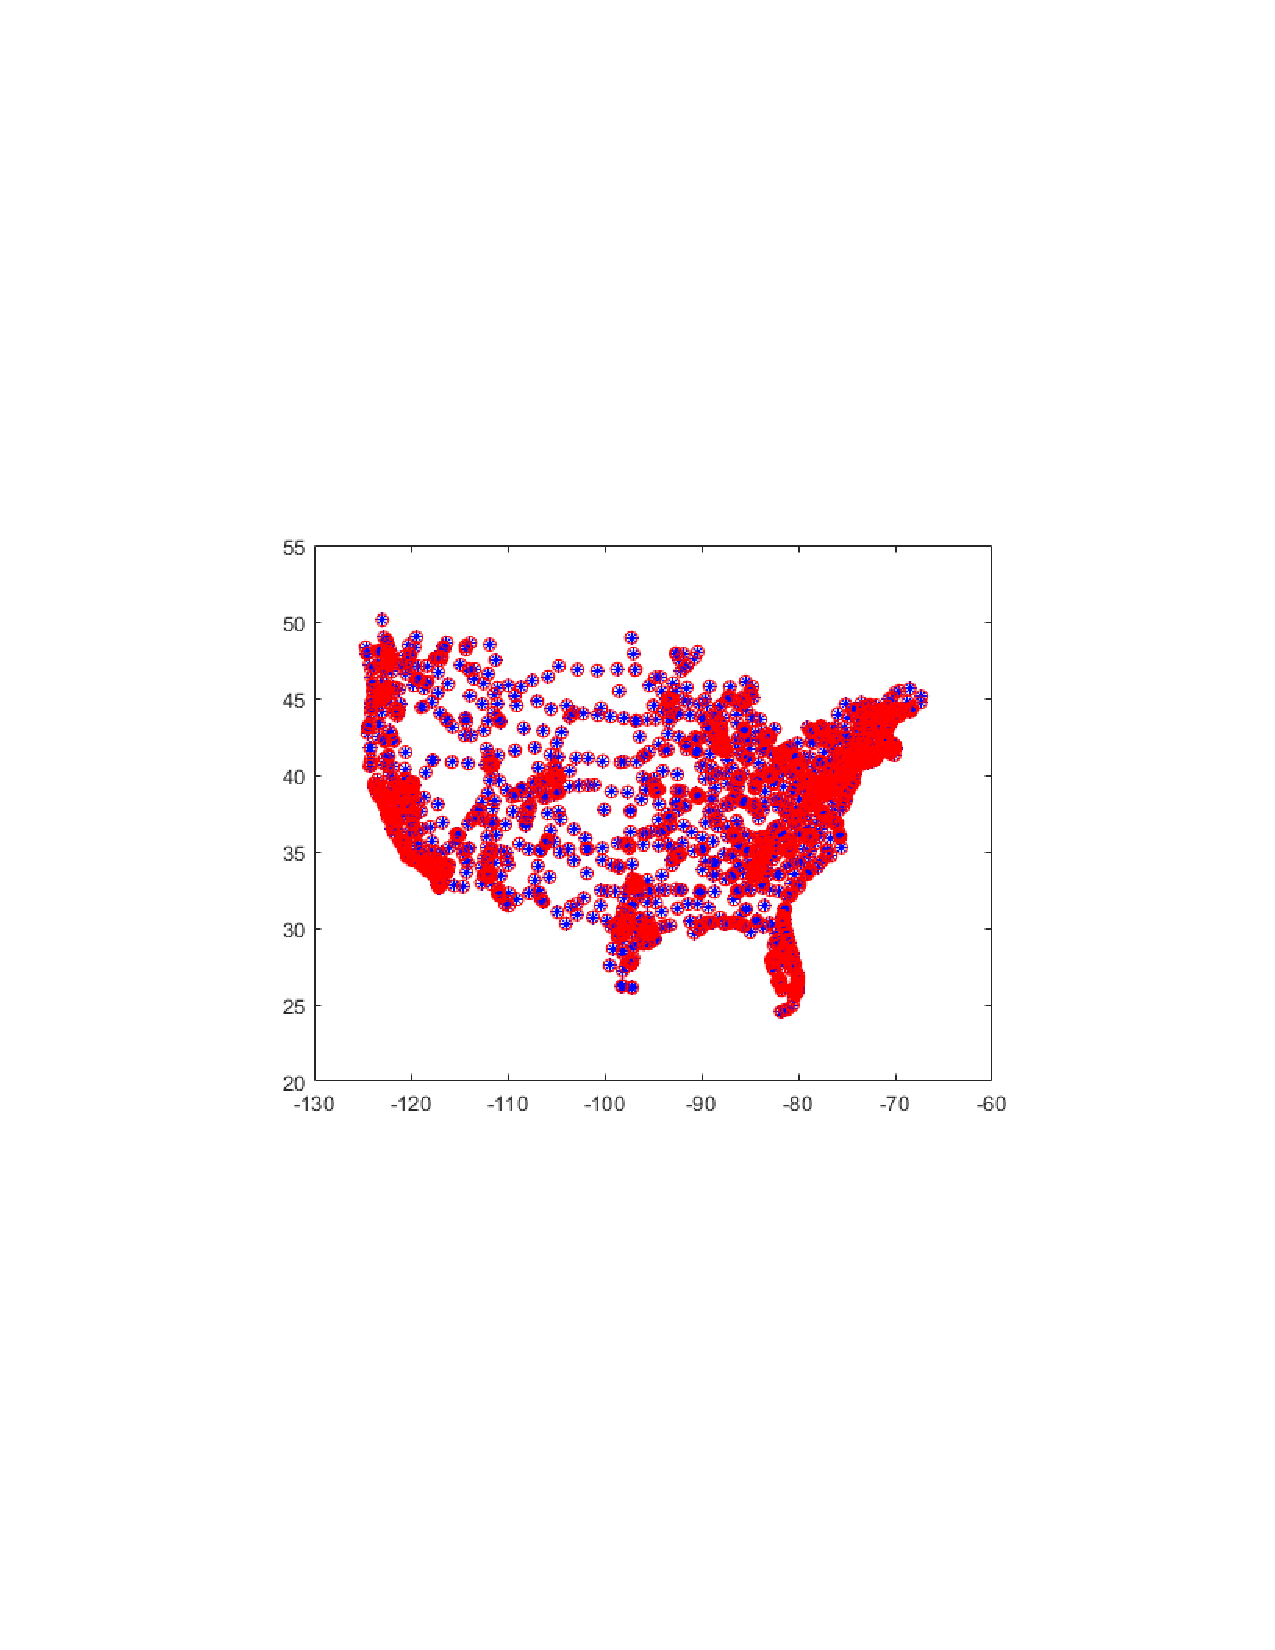
\includegraphics[width=3.2in]{charger_distribution.pdf}
%\vspace{-0.1in}
\caption{The Distribution of Charger Stations in US.}
\label{fig_charger_distribution}
%\vspace{-0.2in}
\end{figure}

\begin{figure}[!t]
\centering
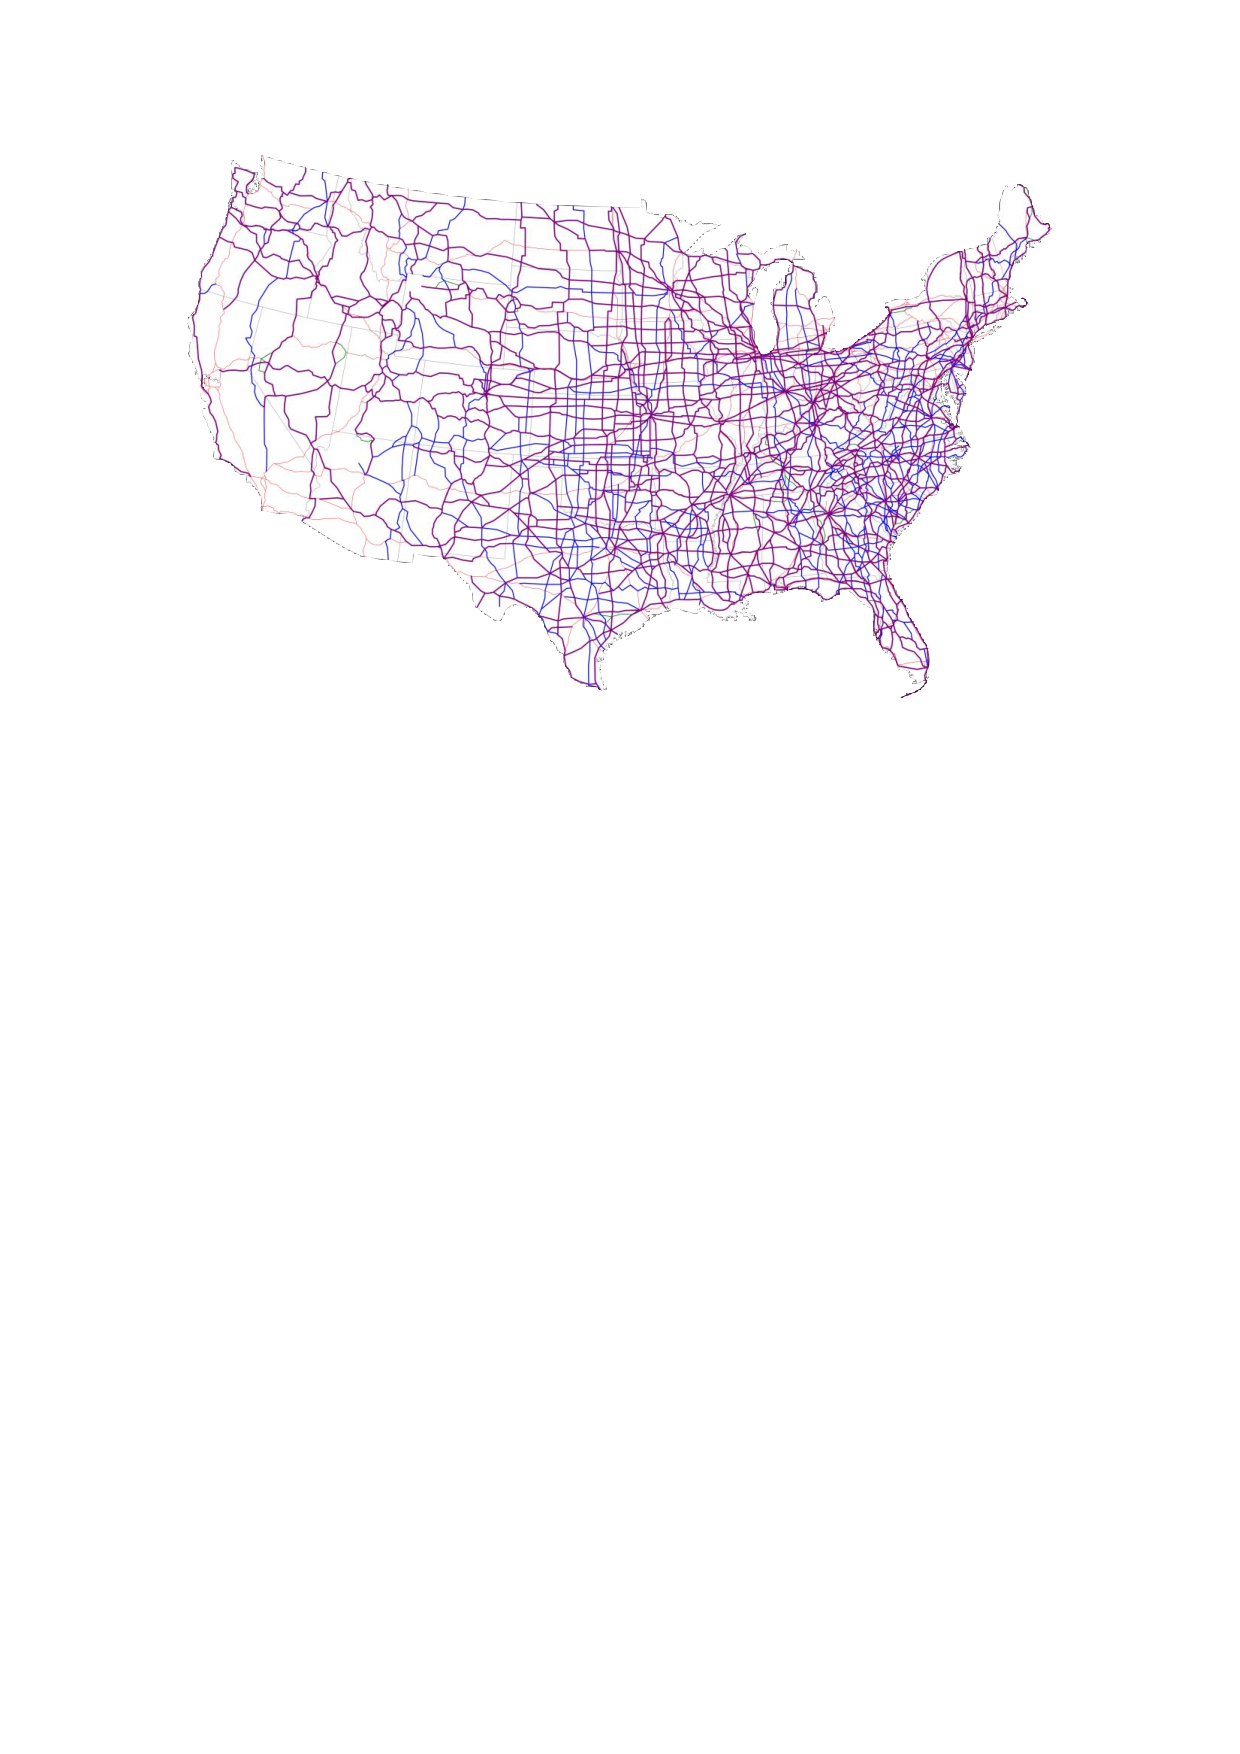
\includegraphics[width=3.2in]{road_map_us.pdf}
%\vspace{-0.1in}
\caption{The Road Map in US.}
\label{fig_road_map}
%\vspace{-0.2in}
\end{figure}

By analysing those data above, we can get three conclusions:
\begin{conclusion}
\label{conclusion_1}
Because of the density of roads, Tesla prefers to construct super charging stations in the area with low density of roads and destination charging station in the area with high density of roads.
\end{conclusion}
\begin{conclusion}
\label{conclusion_2}
As for features of various areas (\eg. urban, suburban, rural area......), Tesla prefers to more super charging stations in suburban and rural area and more destination charging stations in urban.
\end{conclusion}
\begin{conclusion}
\label{conclusion_3}
Tesla plans to deploy more super charging station in area of suburban in the future.
\end{conclusion}

\subsection{The Type of Charging Station}
According to the data above,
A charging station can be seen as a point with four kinds of attributes $sta(x, y, type, R)$.
Specifically, $x$, $y$ are the longitude and latitude of that charging station respectively.
$type$ is its charging type (\eg, destination charging, supercharging),
and $R$ is the maximum driving range provided by $sta(x, y, type, R)$.

Considering supercharging station case,
we find it can provide up to $170$ miles of range~\cite{SuperRange},
so we have $R_{super} = 170miles \approx 272km$.

As for the type of destination charging station,
we consider that it can provide the maximum driving range for an electric vehicle.
Thus, $R_{destination}$ depends on the type of the car.
To simplify our model, withou loss of generality, we assume that our target car is "Tesla Model 3"~\cite{CarRange}.
Considering "Tesla Model 3", the standard maximum range of it is $350km$,
so we have $R_{destination} = 350km$.
As a result, we have:
\begin{equation}
\label{equ_R}
\left\{
\begin{aligned}
& R_{super} = 272km \\
& R_{destination} = 350km \\
\end{aligned}
\right.
\end{equation}

\subsection{The Evaluation of US's Charging Station Network }
To evaluate whether Tesla can support the nation-wide migration of personal transportation to all-electric cars in the United States,
we need to first determine the conditions of a successful migration to all-electric vehicles in the United States.

Note that if the charging stations network can support a successful migration,
an electric vehicle must can get to another charging station from the location of a specific charging station,
so that it would not be restricted in certain area and can travel to anywhere of the whole expected reachable area.

Based on this idea, we can give the conditions of a successful migration to all-electric vehicles in the United States.
\begin{definition}
\label{def_successful_condtion}
\textbf{Successful Switch Condition:}
Suppose that the network of a target area $a$ can support a successful migration to all-electric vehicles,
then for every charing station $sta(x, y, type, R)$ in the network,
it can travel to any other charging station in this network.
\end{definition}

We can model the network as a graph $G_{a}(Vertex, Edge)$.
The set of vertexes $Vertex$ consists of the sites of charing stations.
For a specific site $i$, other sites $j$ that meet the distance $d(i,j) \leqslant R_{type}$ should have an edge $(i,j)$ between them.
All the edge form the set $Edge$.
and the value of a edge can be quantified as the distance.
With Definition~\ref{def_successful_condtion},
it can be considered as the \textbf{Connectivity of the Graph}~\cite{connectivity},
which means if the $G_{a}(Vertex, Edge)$ of area $a$ is a \textbf{Strongly Connected Graph},
then it can support a successful migration to all-electric vehicles in $a$.

Applying the analysis above,
the original problem is now the same as identifying whether the charging station graph $G_{US}(Vertex, Edge)$ of US is a Strongly Connected Graph.
Applying the classic algorithm related to Strongly Connected Graph~\cite{connectivity_algo},
we can reach the conclusion.
\subsubsection{The Result of Evaluation}
By our calculation, note that \textbf{the charging station network in US cannot support a complete switch to all electric}.
The reason of failure is the existence of the kind of case showed in Figure~\ref{fig_failure_case}.
Because $R_{destination} \geq R_{super}$,
there must exists the failure case that the electric vehicle can travel to a super charger station $i$ from a destination charger station $j$, but cannot get back to $j$ from $i$.
Thus, the charing stations network cannot be the Strongly Connected Graph.

In the result of our calculation,
note that there are around 92 this kind of failure in the network,
especially in area between the urban and suburban.
We propose the improvement solution to eliminate this kind of cases showed in Figure~\ref{fig_failure_case}.
Based on the improvement,
we evaluate that \textbf{the total number of charging station that can support a complete switch to all electric is around 3792},
which is higher than the number of current deployment.

\begin{figure}[!t]
\centering
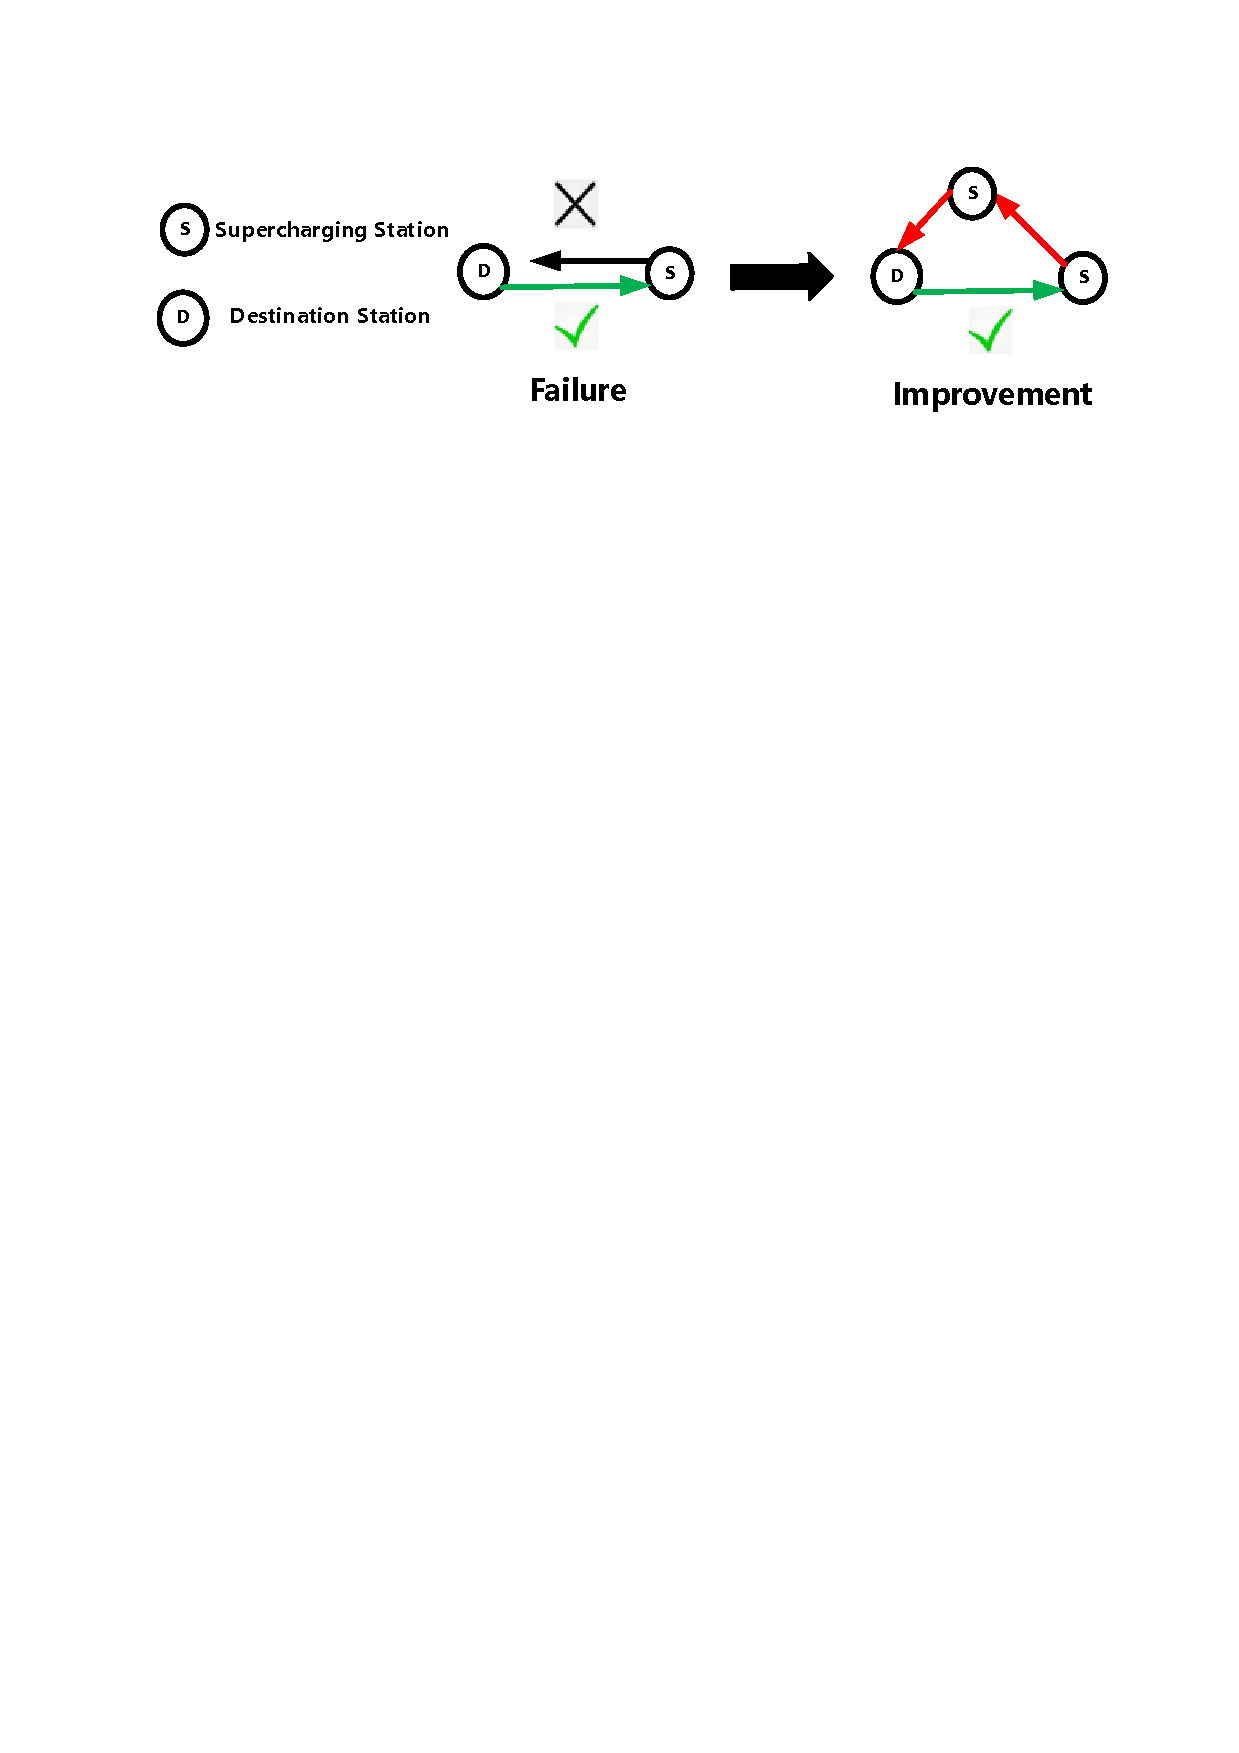
\includegraphics[width=5.2in]{failure_case.pdf}
%\vspace{-0.1in}
\caption{The Case of Failure and Improvement.}
\label{fig_failure_case}
%\vspace{-0.2in}
\end{figure}

\section{Two-Layer Process Architecture}
\label{sec_system_architecture}
Based on Section~\ref{sec_profile_us}, we find there too many factors to consider thus make problem too complex to solve. 
Thus, we propose a \textbf{two-layer process architecture} to simplify the problem without loss of generality.

In this section, we give a brief introduction to the two-layer process architecture we used to process this problem.
The main idea of this two-layer process architecture is to divide the whole problem into two dimension (\ie, Selection and Optimization).
Thus, we can classify various factors into two different layers so that we can simplify our model without loss of generality and make it solvable.
Figure 5 illustrates the Two-Layer Process Architecture in our paper.
\subsection{Selection Layer}
In Selection Layer,
the main task is to select the potential sites for charging stations.
This part mainly depends on many external factors (\eg, different geographies, population density, wealth distribution, policy of the government, area's type......).
Thus, we can just consider those factors in this layer.
After process, this layer should output the set of potential sites which can construct charging station.
%When we are trying to determine a specific location for constructing a new charing station within urban area, several potential locations have to be determined in the first place.
%A schematic elaborating this 2 step process has been depicted as follows.

\begin{figure}[!t]
\label{fig_system_architecture}
\centering
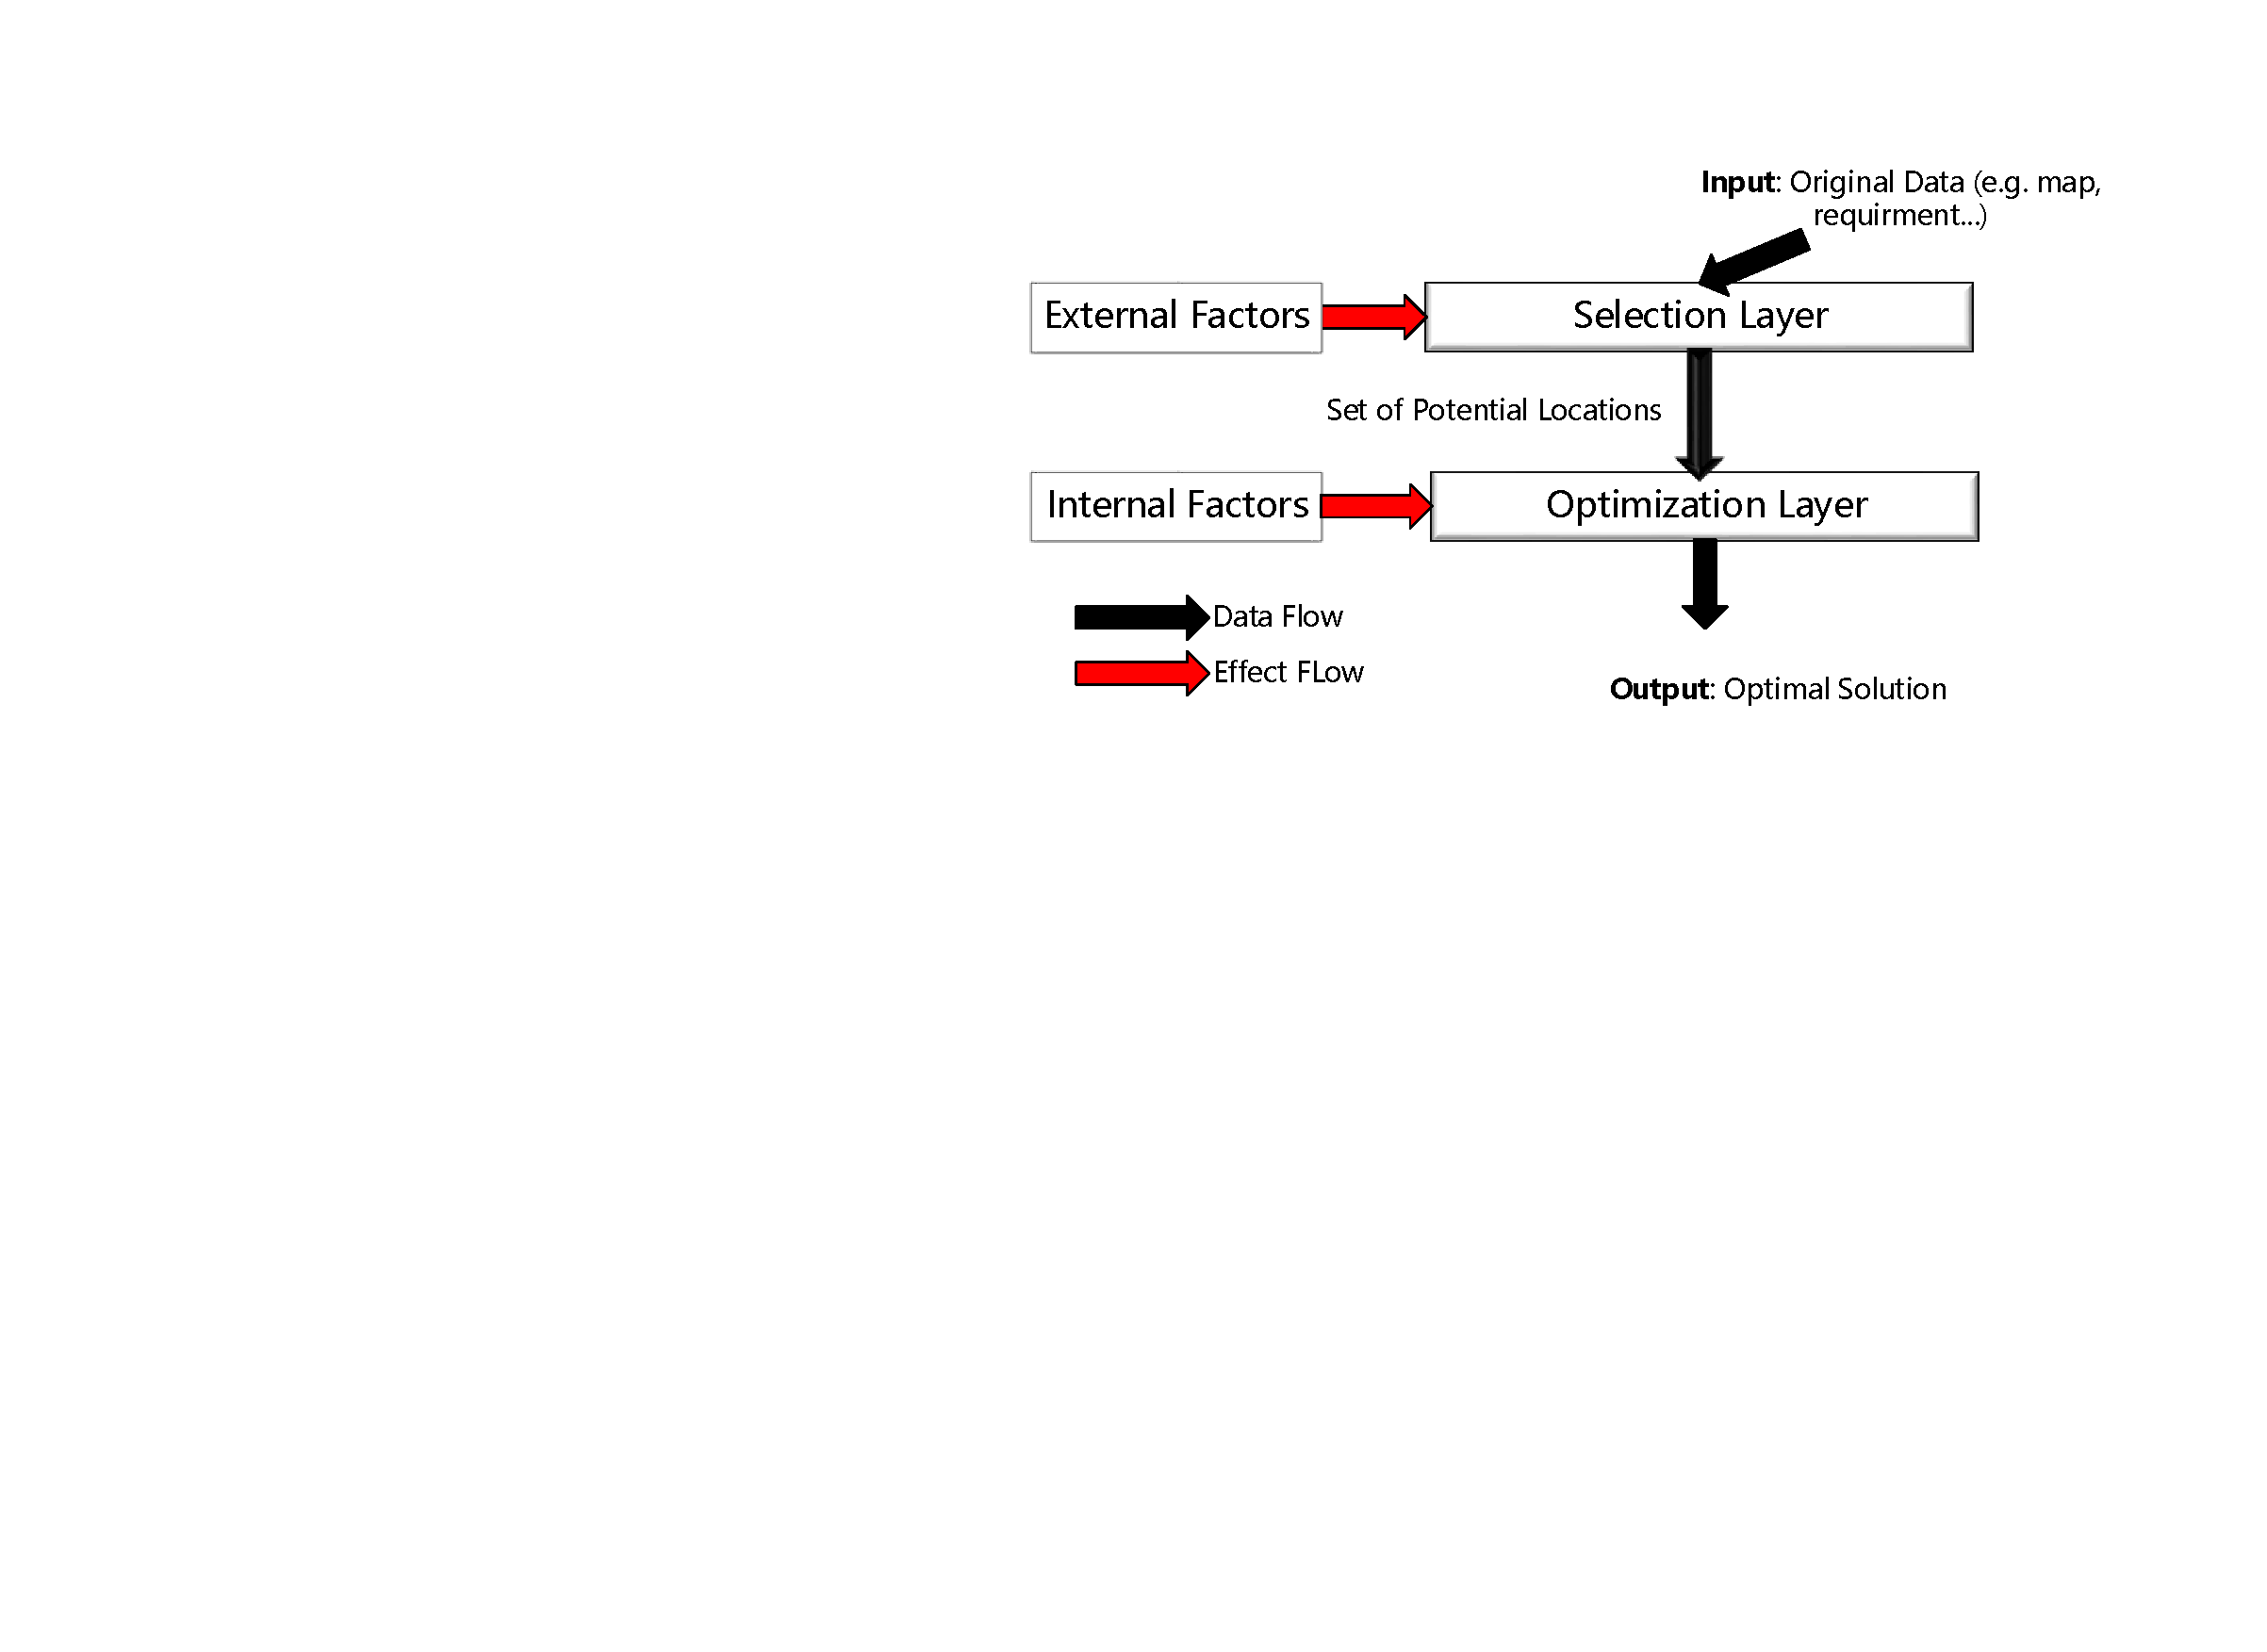
\includegraphics[width=4in]{system_architecture}
%\vspace{-0.1in}
\caption{Two-Layer Process Architecture}
%\vspace{-0.2in}
\end{figure}


\subsection{Optimization Layer}
In Optimization Layer,
the main task is to find the optimal number, placement, and distribution of charging stations based on the result from Selection Layer.
Since the set of potential sites is decided in Selection Layer,
according to the algorithm we designed in Section~\ref{sec_solve_optimal}, 
Optimization Layer just choose some sites of the set to achieve the optimal performance.
The algorithm depends on some internal factors (\eg, charging demand, the habit of drivers, connection of roads, service capacity of the charging station).
Therefore, we just consider those internal factors in this layer.

%root=main.tex
\section{System Model}
\label{sec_basic_model}

We build the basic model of a charging station,
and analyze whether or not Tesla can support a successful migration to all-electric personal transpotations in the United States from the energy perspective.

\subsection{The Standard of Feasibility}
\label{subsec_standard_feasibility}
In order to evaluate the feasibility of supporting a successful migration to all-electric personal transpotations in the United States,
we firstly need to define feasibility.
\begin{definition}
\textbf{Solution Feasibility:}
\label{def_feasibility}
Suppose $Solution(a)$ is the solution of the target area $a$,
the solution of charging stations is feasible if and only if:
(1) it can meet the \textbf{charging demand} in target area $a$,
(2) it can let the vehicle get to anywhere (\textbf{coverage}) in target area $a$.
\end{definition}
In Definition~\ref{def_feasibility}, coverage can be regarded as the Connectivity of the networking graph in area $a$ mentioned in Section~\ref{sec_profile_us},
but it is hard to quantify the charging demand in area $a$.
To solve this issue,
we refer to the previous work about the layout of electric vehicle charging station~\cite{wang2010novel},
Note that it is reasonable to quantify the charging demand from the energy perspective.
Here is the definition of the charging demand.
\begin{definition}
\textbf{Charging Demand:}
\label{def_charging_demand}
Suppose $Demand(a)$ is the charging demand of the target area $a$,
$R_{electic}(a)$ is the penetration rate of electric vehicles in target area $a$,
and $E_{consume}(a)$ is the energy consumed by traffic of $a$,
then we have the equation:
\begin{equation}
\label{equ_demand}
Demand(a) = E_{consume}(a) \times R_{electric}(a)
\end{equation}
\end{definition}
Suppose the set of the charging stations in $a$ is $Set(a)$,
$Set_i(a)$ represents a specific charging station $i$ and the energy it can provide is $E(Set_i(a))$.
If and only if the solution can meet the equation:
\begin{equation}
\label{equ_energy}
\sum{E(Set_i(a))} (i \in Set(a)) \geqslant Demand(a)
\end{equation}
Then, we say the solution can meet the charging demand of target area $a$.

For the distribution of charging demand in target area $a$,
without considering its shape, we suppose the leaving vehicles and the entering vehicles are equal in quantity,
then the number of the vehicles in area $a$ should be a constant, denoted as $N_{a}$.
This factor should depends on \textbf{population density} and \textbf{wealth condition}(the electric vehicle penetration rate $R_{electic}(a)$) of $a$.

%\subsection{The Model of Charger Station}


%We suppose the size of coverage area that a specific charging station can provide is circle.
%Thus, we can calculate the coverage area sizes of destination charging and supercharging respectively:


\subsection{The Model of City}
For the model of the city,
we treat a city $a$ as an undirected graph $G_{a}(Po(a),\theta(a))$.
This idea has been proved to be reasonable by the work~\cite{lam2014electric}.
Specifically, $Po(a)$ denotes the set of possible sites for constructing charging station,
and $\theta(a)$ denotes the set of roads connecting pairs of sites.
Let $d(i, j)$ denotes the distance of the shortest path from $i$ to $j$ by traversing the roads in $\theta(a)$,
which can be calculated by Dijkstra's Algorithm~\cite{Dijkstra}.
Note that, here $d(i, j)$ refers to the distance of an actual road connecting sites $i$ and $j$ but not the Euclidean distance.

Each site $i$ has a charging demand requirement $Demand(i)$ which is defined in Definition~\ref{def_charging_demand}
(\eg, the more electric vehicles in the coverage of the charging station located in $i$, the higher $Demand(i)$ is).
Let $Cap(i)$ be the capacity of node $i$ which represents the average capacity of charging service supported if a charging station is constructed at location $i$.

Considering the City model above, we can give the definition of the reachability.
\begin{definition}
\label{def_reachability}
\textbf{Reachability:}
Suppose $G_{a}(Po(a),\theta(a))$ is the graph of area $a$,
$Po(a)^{'}$ is the subset of $Po(a)$,
then we say anywhere in $Po(a)^{'}$ is reachable if and only if it can follow three conditions below:
\begin{condition}
\label{con_reach_1}
$\forall i \in Po(a)^{'} \Rightarrow \exists j \in Po(a)^{'},  d(i, j) \leqslant R$
\end{condition}
\begin{condition}
\label{con_reach_2}
$\forall i \in Po(a), Cap(i) = \sum{Cap(j)}, (j \in Po(a)^{i}, d(i, j) \leqslant \alpha{R}) \Rightarrow Cap(i) \geqslant Demand(i)$
\end{condition}
\begin{condition}
\label{con_reach_3}
$\forall i, j \in Po(a)^{i} \Rightarrow d(i, j)  \leqslant n_{ij}R, (n_{ij} \geqslant 1)$
\end{condition}
(Note that $\alpha \in (0,1]$ is the factor to describe the habit of recharging of drivers,
 $n_(ij)$ represents the amount of charging stations along the path $d(i, j)$)
\end{definition}

Condition~\ref{con_reach_1} means that any charging station in a specific location can recharge at another site within the range $R$,
which guarantees that any electric vehicle would not be restricted in one area.

Condition~\ref{con_reach_2} means that the local charging demand at a area must be satisfied by the total charging capacities contributed by those charging stations located within distance $\alpha{R}$ away.
Here, we use the factor $\alpha$ represents the habit of recharging of drivers.
(\eg, $\alpha = 0.75$ means that the driver would recharge the vehicle when the vehicle has consumed $75\%$ of the total energy.)

Condition~\ref{con_reach_3} says, in the charging station network, the vehicle can go by more than one charging stations to travel to another charging station.

In order to explain our model more clearly,
Figure~\ref{fig_city_model} shows a simple example of our model based on Los Angeles~\cite{LAMap}.


\begin{figure}[!t]
\centering
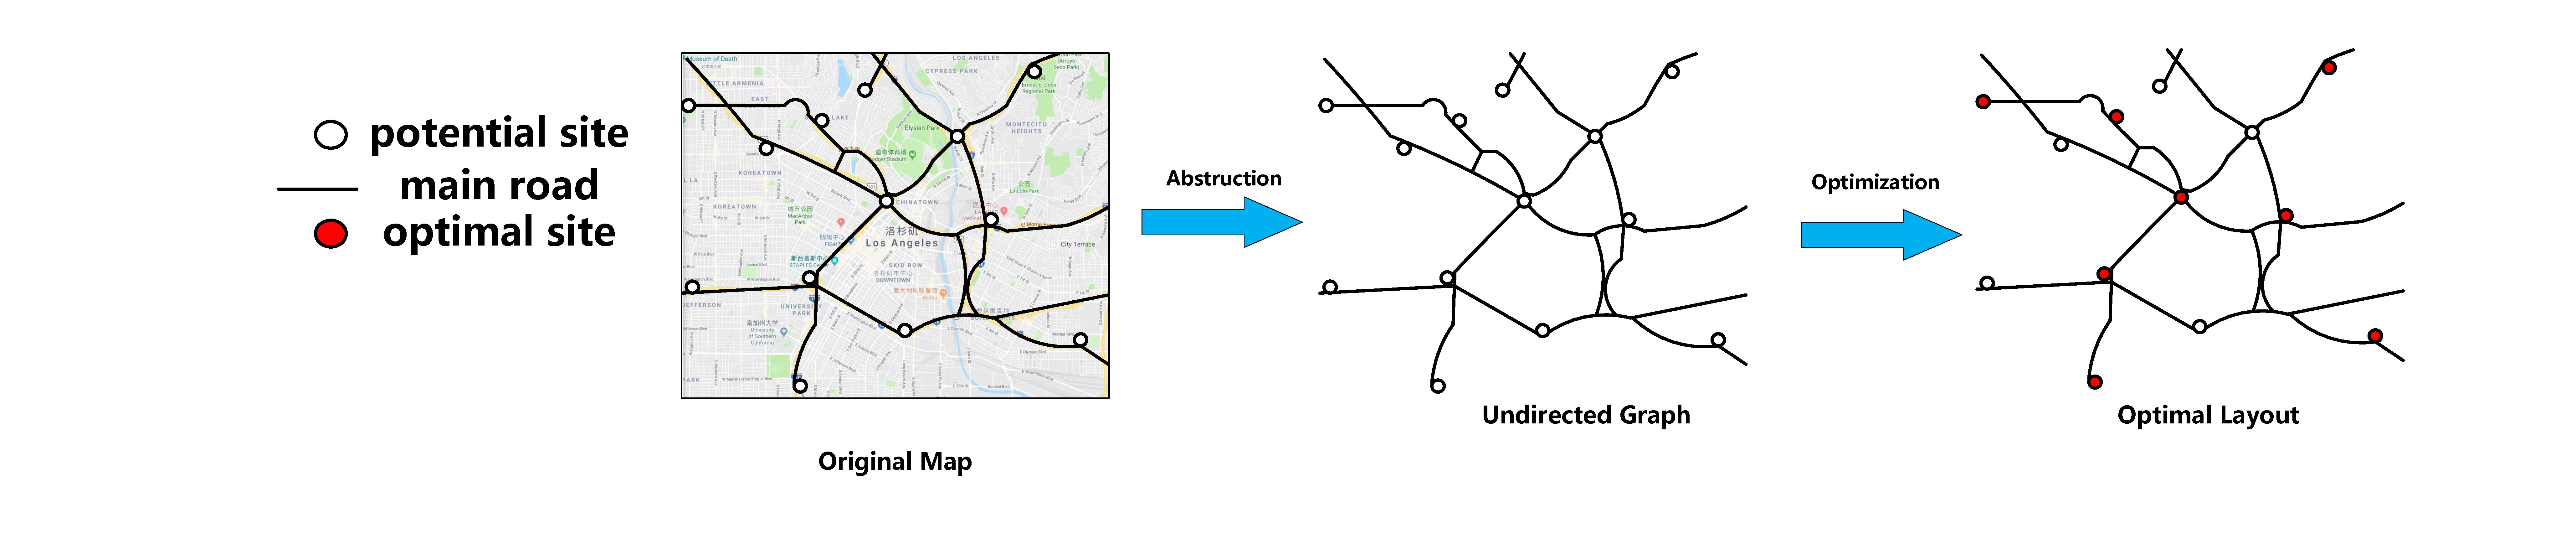
\includegraphics[width=6.7in]{city_model.pdf}
%\vspace{-0.1in}
\caption{An Example of our City Model.}
\label{fig_city_model}
%\vspace{-0.2in}
\end{figure}


\section{Problem Formulation}
\label{sec_problem_formulation}
In this section, we shows how we formalize the problem of determining the optimal number, placement and distribution of charging station.
\begin{definition}
\label{def_optimal}
\textbf{Optional Distribution:}
Suppose area $a$ is the target area and its graph is $G_{a}(Po(a),\theta(a))$,
the Optional Distribution for $a$ is the solution $\varsigma(a)$ that can meet conditions mentioned in Definition~\ref{def_reachability} and make $a$ is reachable with minimal cost.
\end{definition}
We suppose $X=[x_0, x_1, ......,x_i,......,x_n]$ is a vector, $x_i$ represents the decision of site $i$,
and the value of $x_i$ is defined as:
\begin{equation}
\label{equ_decision_x_i}
x_i =\left\{
\begin{aligned}
& 0 \quad \text{the site $i$ is not used}\\
& 1 \quad \text{the site $i$ is used}\\
\end{aligned}
\right.
\end{equation}
Because we assume the task of optimization belongs to Optimization Layer (the second layer) in Section~\ref{sec_system_architecture},
the input of this problem is the set of potential sites calculated by Selection Layer (the first layer) in our two-layer process architecture.

Suppose the cost of constructing charging station in site $i$ is $c_i$,
then, the total cost of the a solution $\varsigma(a)$ in area $a$ is $Cost_{\varsigma(a)}$,
\begin{equation}
\label{equ_cost}
Cost_{\varsigma(a)} = \sum_{i=0}^{n}x_i \times c_i
\end{equation}
We regard Equation~\ref{equ_cost} as the objective function need to minimize.
After the formulation of the objective function,
we also need to formulate those three conditions mentioned in Definition~\ref{def_reachability}.
\subsection{Condition Formulation}
Because Condition~\ref{con_reach_1} is contained in Condition~\ref{con_reach_3}.
We do not demonstrate it in detail here.

In order to formulate Condition~\ref{con_reach_2} more clearly,
we introduce $Set^{\alpha{R}}(i)$.
For each $i \in Po(a)$
\begin{equation}
Set^{\alpha{R}}(i)=\{j \in Po(a) | d(i,j) \leqslant \alpha{R} \}
\end{equation}
Then, the Condition~\ref{con_reach_2} is equivalent to the equation below,
\begin{equation}
\label{equ_condition_2}
\sum_{j \in Set^{\alpha{R}(i)}} Cap(j) \times x_j \geqslant Demand(i)
\end{equation}

For Condition~\ref{con_reach_3},
it is hard to be formulated directly and we refer to the idea in the work~\cite{lam2013electric}.
We firstly need to generate a graph $G_{a}^{'}({Po}^{'}(a),{\theta}^{'}(a))$ of area $a$,
Specially, ${Po}^{'}(a)$ is set to $Po(a)$ and ${\theta}^{'}(a)$ is defined as:
\begin{equation}
\label{equ_G'}
{\theta}^{'}(a) =\{(i,j) | i,j \in Po(a), d(i,j) \leqslant R, i \neq j \}
\end{equation}
Figure~\ref{fig_graph_example} illustrates an example with $R = 6$ and a 6-node graph,
with the Equation~\ref{equ_G'}, we can generate $G^{'}$ from $G$.
the number on a edge indicates the distance between the nodes on the two ends,
and the number in the circle is the id of the node.
In other words, those nodes i in $G$ with $x_i = 1$ constitute the corresponding induced subgraph~\cite{Induced_Subgraph} $G{'}_{sub}$ of $G^{'}$.
Therefore, we consider that Condition~\ref{con_reach_3} is equivalent to existing \textbf{induced subgraph connected},
and we can use $G^{'}$ to define the problem instead of $G$.
\begin{figure}[!t]
\centering
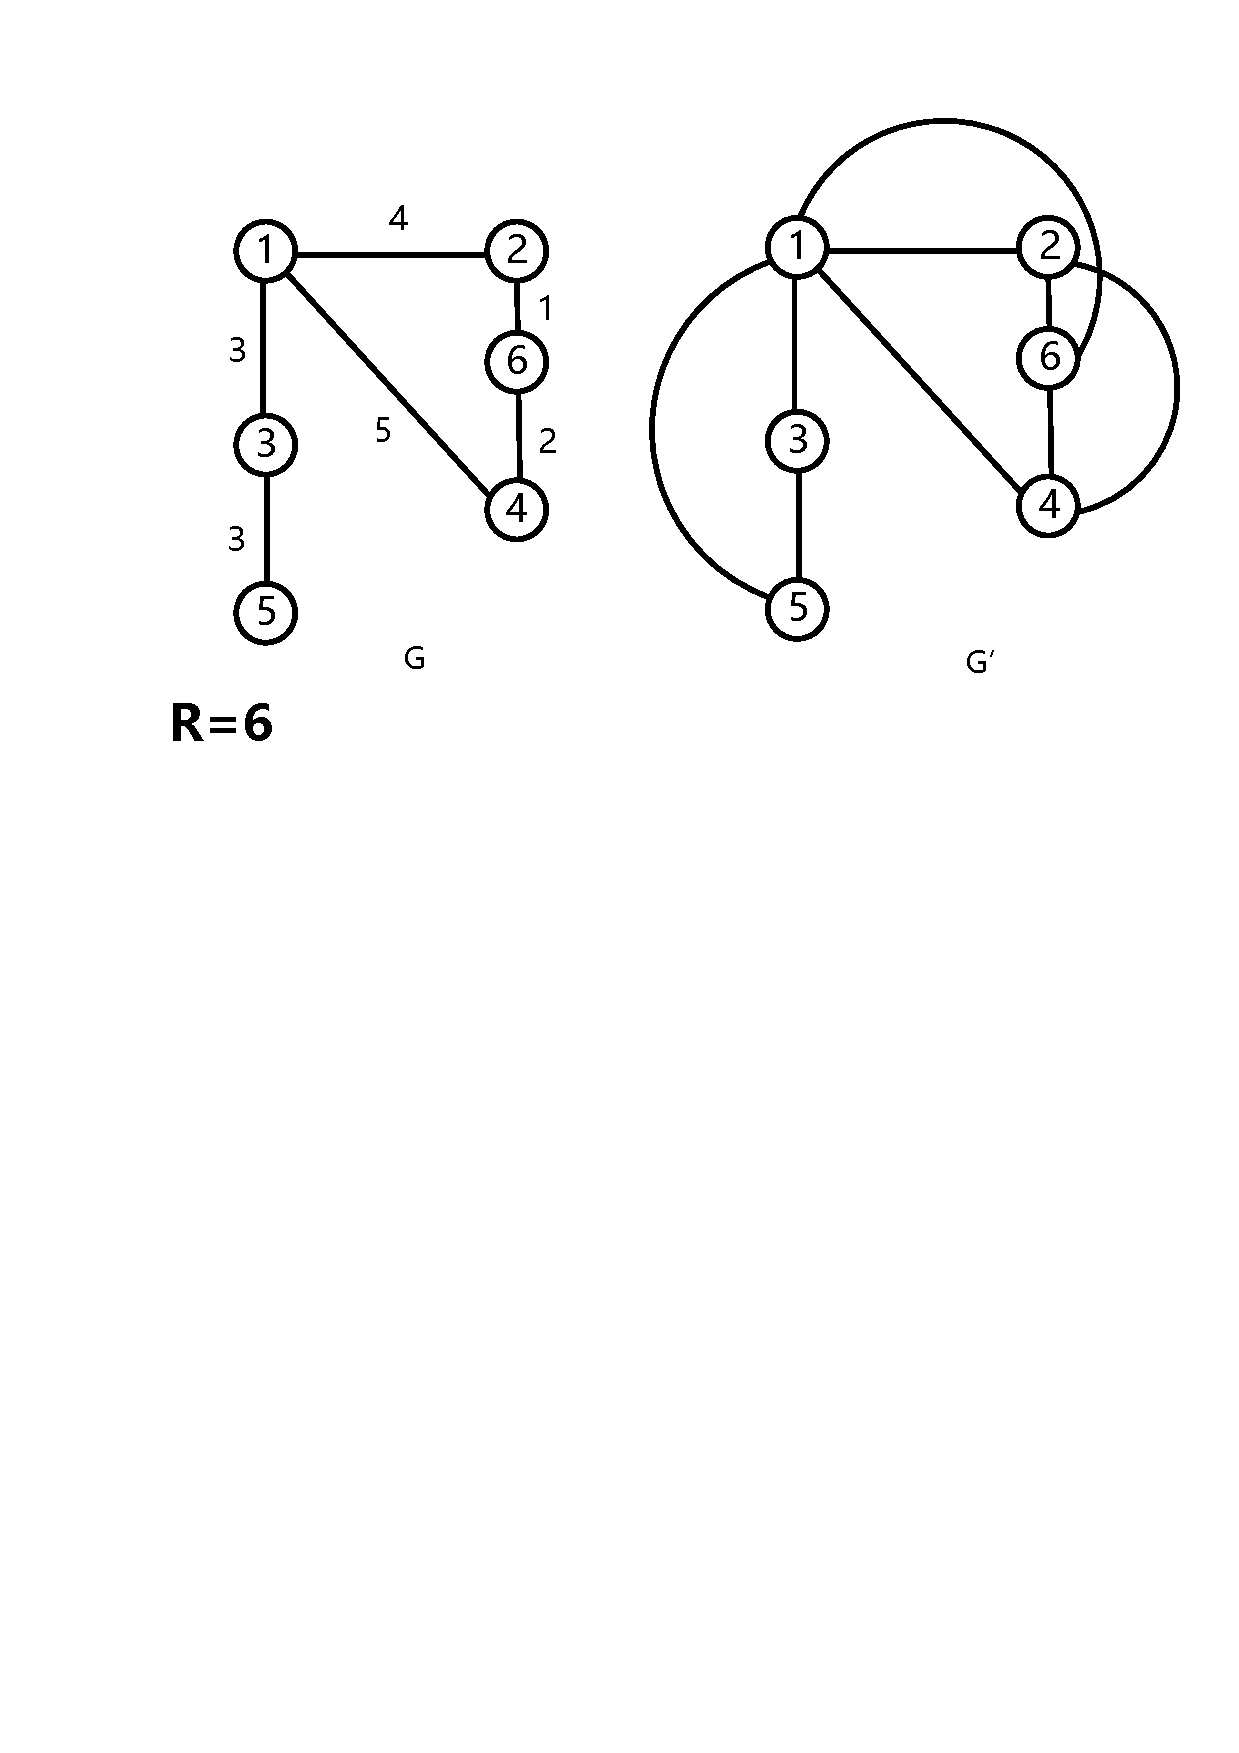
\includegraphics[width=3.5in]{graph_example.pdf}
%\vspace{-0.1in}
\caption{A 6-node Example of $G_{a}(Po(a),\theta(a)) \rightarrow G_{a}^{'}({Po}^{'}(a),{\theta}^{'}(a))$ .}
\label{fig_graph_example}
%\vspace{-0.2in}
\end{figure}

To formulate the problem regarding to induced subgraph, we use the network flow model in the work~\cite{conrad2012wildlife, lam2014electric}.
Suppose there is a source node $0_i$ attached by another node $i$,
the source node $0_i$ has $n$ units of flow available to be sent along $G^{'}$ through node $i$.
Suppose $Surplus_0$ represents the units not consumed by the network in source node $0_i$.

For each node $j$ with $x_j = 1$, it consumes one unit of flow.
Suppose the edge $e(j,k) \in {\theta}^{'}(a)$,
the amount of unit on $e(j,k)$ originated from $0_i$ is $V^{i}_{e(j,k)}$
then, to guarantee those nodes $j$ with $x_j=1$ being reached from node $i$ on $G^{'}$ (site $i$ has been selected as one of charging stations),
it should follow equations below:
\begin{equation}
\label{equ_condition3_equation}
\left\{
\begin{aligned}
& Surplus_0+V^{i}_{e(0,i)} = n,     \\
& 0 \leqslant V^{i}_{e(j,k)} \leqslant nx_k, \forall e(j,k) \in {\theta}^{'}(a)\bigcup e(0_i, i)  \\
& \sum_{j \in {Po}^{'}(a)}x_j = V^{i}_{e(0,i)}\\
& \sum_{j \in {Po}^{'}(a), e(j,k) \in {\theta}^{'}(a)} V^{i}_{e(0,k)} = x_k + \sum_{l \in {Po}^{'}(a), e(k,l) \in {\theta}^{'}(a) } V^{i}_{e(k, l)}, k \in Po^{'}(a) \\
& Surplus_0 \geqslant 0\\
\end{aligned}
\right.
\end{equation}

Note that, in equations above,
we assume $i$ is the only node that attached with the source in this network, which means the electric vehicle charged in $i$ can achieve any node in the network.
However, according to real requirement of this problem, $\forall i \in Po^{'}(a)$ can be attached with the source,
which means if a specific electric vehicle is charged in any charging station in the network,
it can achieve any other charging station.
Thus, we should extend the Equation~\ref{equ_condition3_equation} to the case that $\forall i\in P^{'}(a)$.

With Equation~\ref{equ_cost}, Equation~\ref{equ_condition_2} and Equation~\ref{equ_condition3_equation},
we can summary the problem of finding optimal solution as follows:
\begin{problem}
\textbf{Optimal Problem:}
\label{pro_optimal}
\begin{equation}
\label{equ_final}
\begin{split}
&\text{\textbf{Objective.} minimize the function: }Cost_{\varsigma(a)} = \sum_{i=0}^{n}x_i \times c_i \\
&\text{\textbf{Constraints.}}\left\{
\begin{aligned}
& \sum_{j \in Set^{\alpha{R}(i)}} Cap(j) \times x_j \geqslant Demand(i) \\
& Surplus_0+V^{i}_{e(0,i)} = n,     \\
& 0 \leqslant V^{i}_{e(j,k)} \leqslant nx_k, \forall e(j,k) \in {\theta}^{'}(a)\bigcup e(0_i, i)  \\
& \sum_{j \in {Po}^{'}(a)}x_j = V^{i}_{e(0,i)}\\
& \sum_{j \in {Po}^{'}(a), e(j,k) \in {\theta}^{'}(a)} V^{i}_{e(0,k)} = x_k + \sum_{l \in {Po}^{'}(a), e(k,l) \in {\theta}^{'}(a) } V^{i}_{e(k, l)}, k \in Po^{'}(a) \\
& Surplus_0 \geqslant 0\\
\end{aligned}
\right.
\end{split}
\end{equation}
\end{problem}

\section{The Method to Solve the Optimal Problem}
\label{sec_solve_optimal}
In this section, we apply the Algorithm 1 to solve Equation~\ref{equ_final}.
Our algorithm is based on Greedy Algorithm~\cite{Greedy_Algorithm}.
We suppose the input of this algorithm is the graph of the target area $a$ and the set of cost $C_{set}$ consists $c_i, i \in Po^{'}(a)$,
and the graph of the target area $a$ can be generated by the first layer after it processed the original map of target area.
The output of this algorithm is the decision vector that can determine the set of nodes that should be used as the site to construct charging stations.
Algorithm~\ref{alg_solve_optimal} summaries the process of our algorithm.
\begin{algorithm}
\label{alg_solve_optimal}
\small
\caption{{\tt Find\_Optimal\_Solution}($G^{'}_{a}(Po^{'}(a),\theta^{'}(a))$, $C_{set}$)}
\KwIn{$G^{'}_{a}(Po^{'}(a),\theta^{'}(a))$: the graph of target area $a$, \\
$C_{set}$ is the set of cost, $c_i \in C_{set}$ represents the cost of constructing a charging station in site $i$.}
\KwOut{$X$: the vector, $x_i$ is defined in Equation~\ref{equ_decision_x_i}.}
Initialize the vector $X$: Set the length of $X$ equals to the number of elements in $Po_(a)$, the default value of $x_i, i \in Po^{'}_{a}$ is $1$\;
Construct a temporary node set $N_{temp}$of nodes $i$ with $x_i = 1$,
where the induce subgraph is still connected when $x_i$ is set to 0\;
\While{$N_{temp} == \text{NULL}$}{
    $X^{'} \leftarrow X$\;
    $flag \leftarrow 0$\;
    \While{$flag == 0 $ OR $N_{temp} == \text{NULL}$}{
        Select $j$ with the largest $c_i, i \in N_{temp}$\;
        Change $X^{'}$ with $x^{'}_j \leftarrow 0$\;
        \eIf{$X^{'}$ meets $\sum_{j \in Set^{\alpha{R}(i)}} Cap(j) \times x_j \geqslant Demand(i)$}{
                        $X \leftarrow X^{'}$\;
                        $flag \leftarrow 1$\;
                }
                {
                        $x^{'}_j \leftarrow 1$\;
                        Delete $j$ in $N_{temp}$\;
                }
    }
}
\Return {$X$}\;
\end{algorithm}
\begin{figure}[h]
\centering
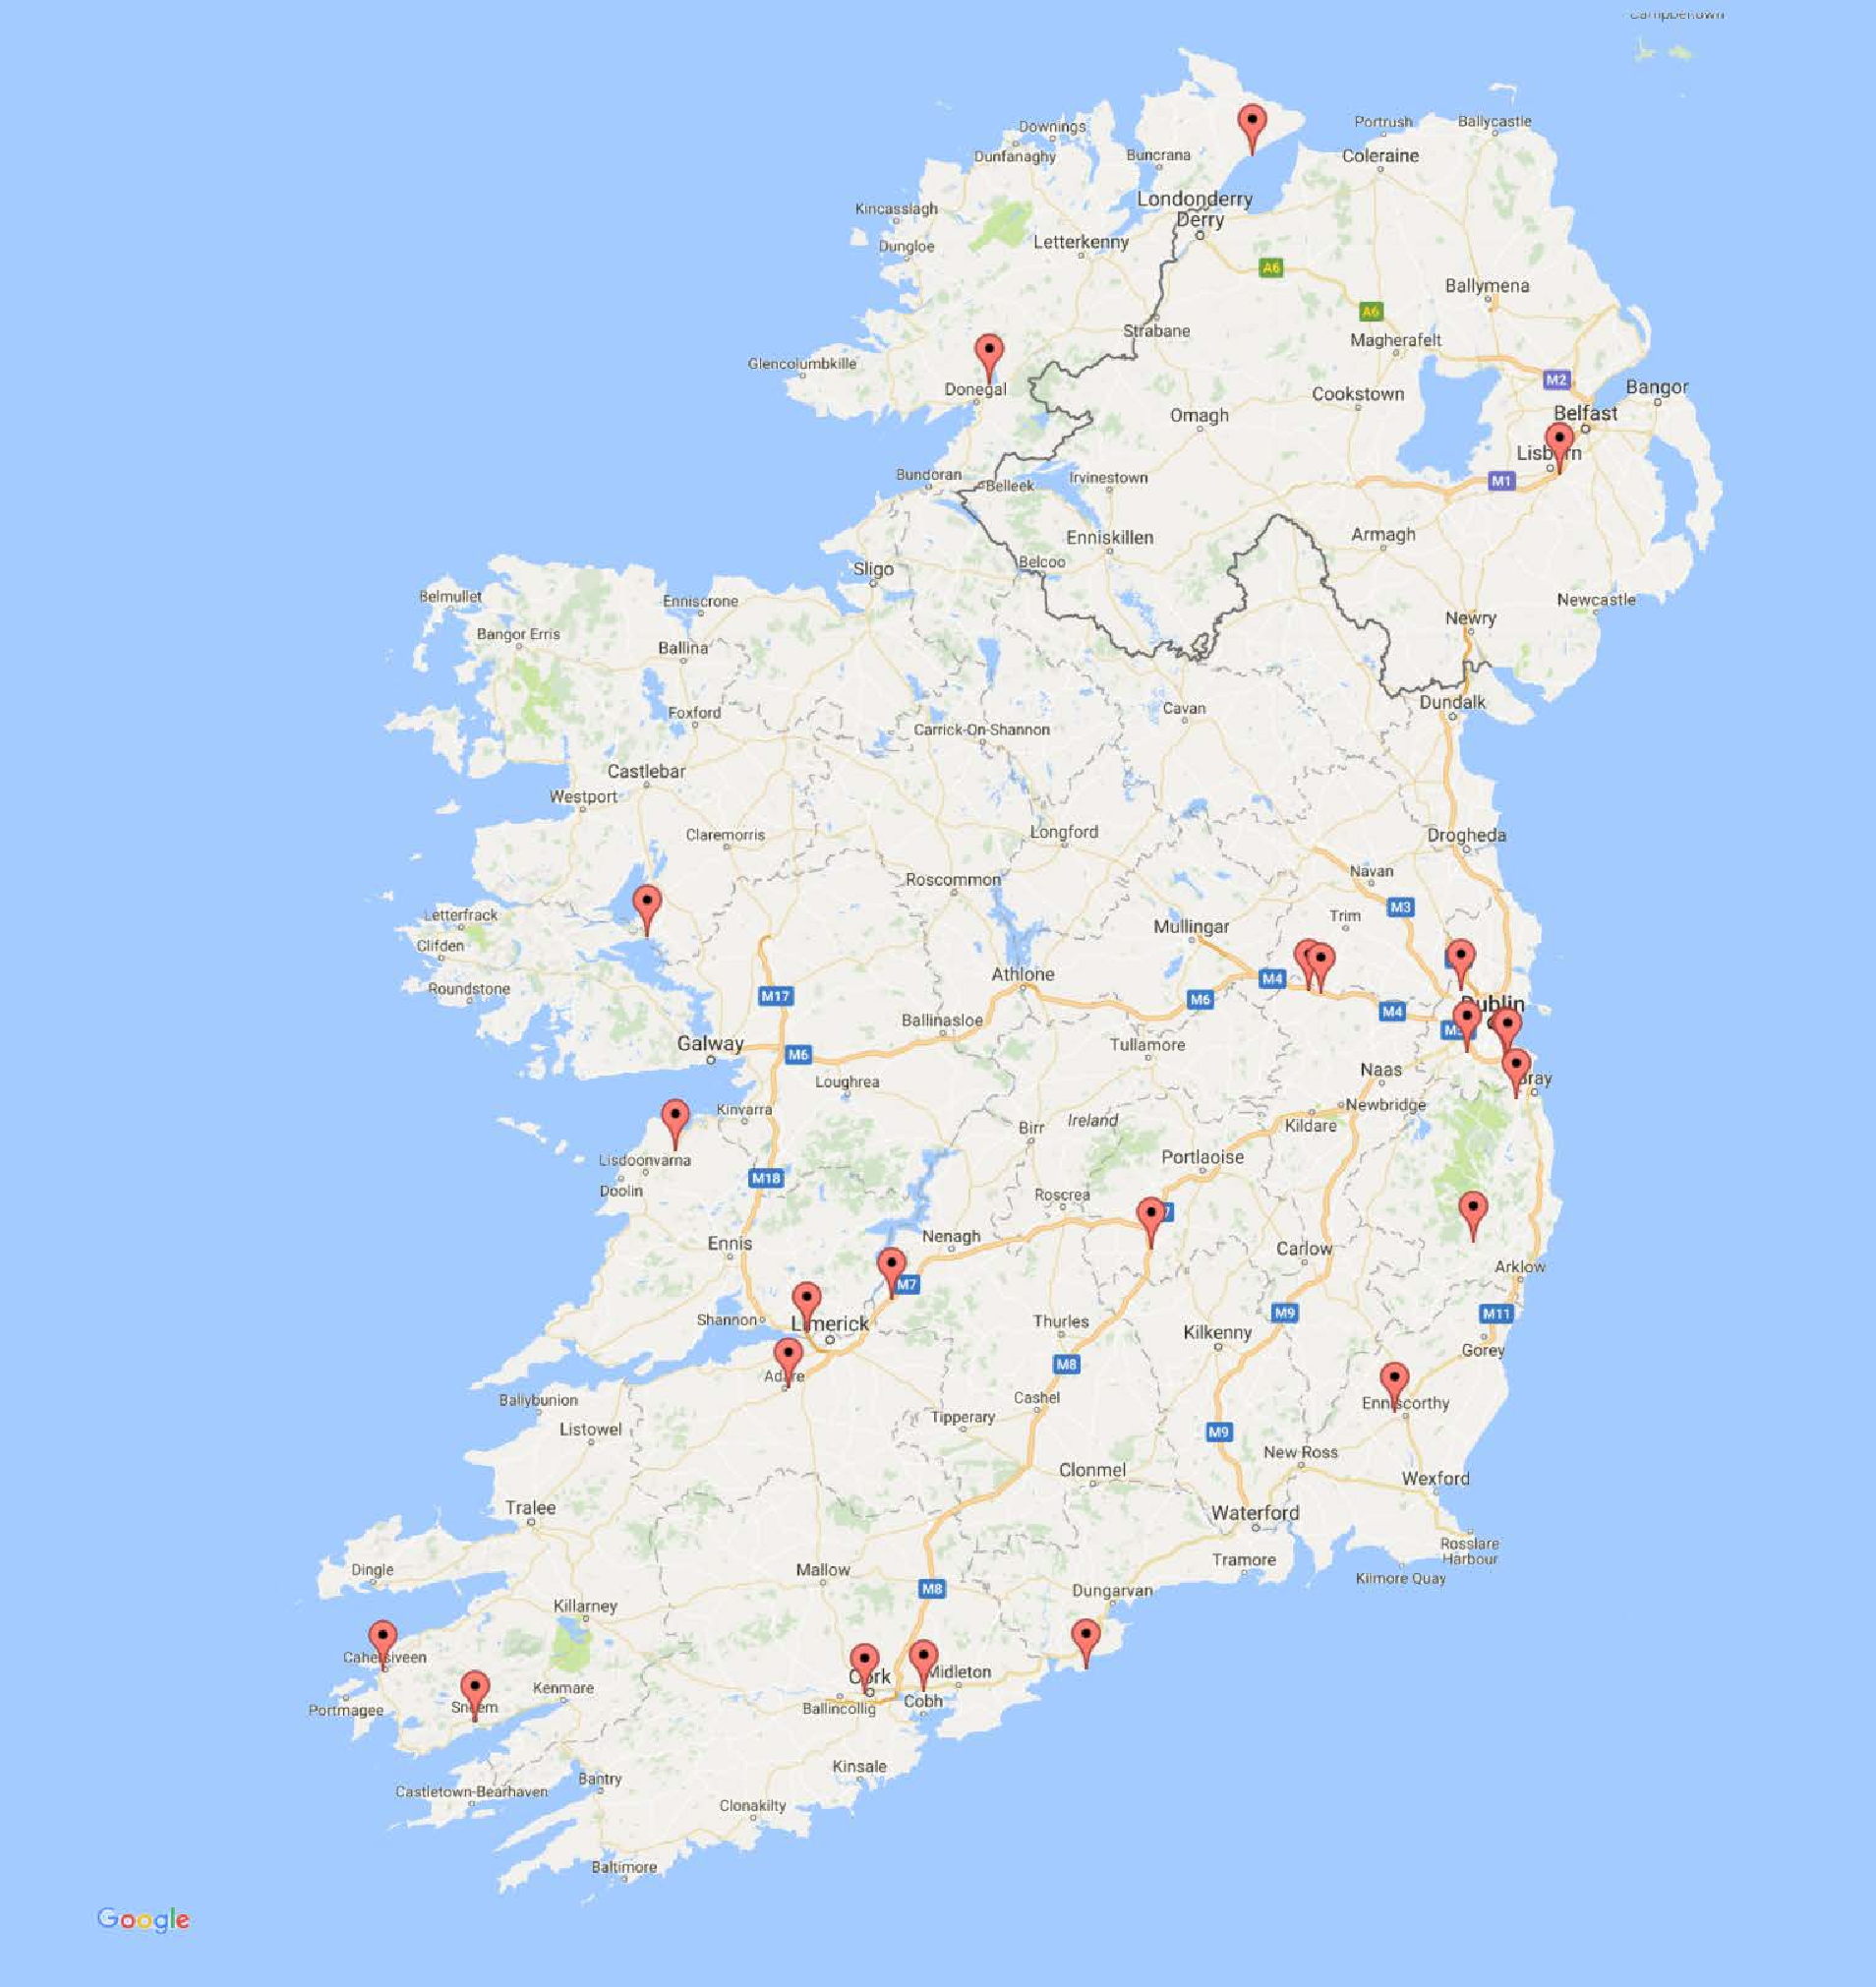
\includegraphics[width=2in]{stage0.pdf}
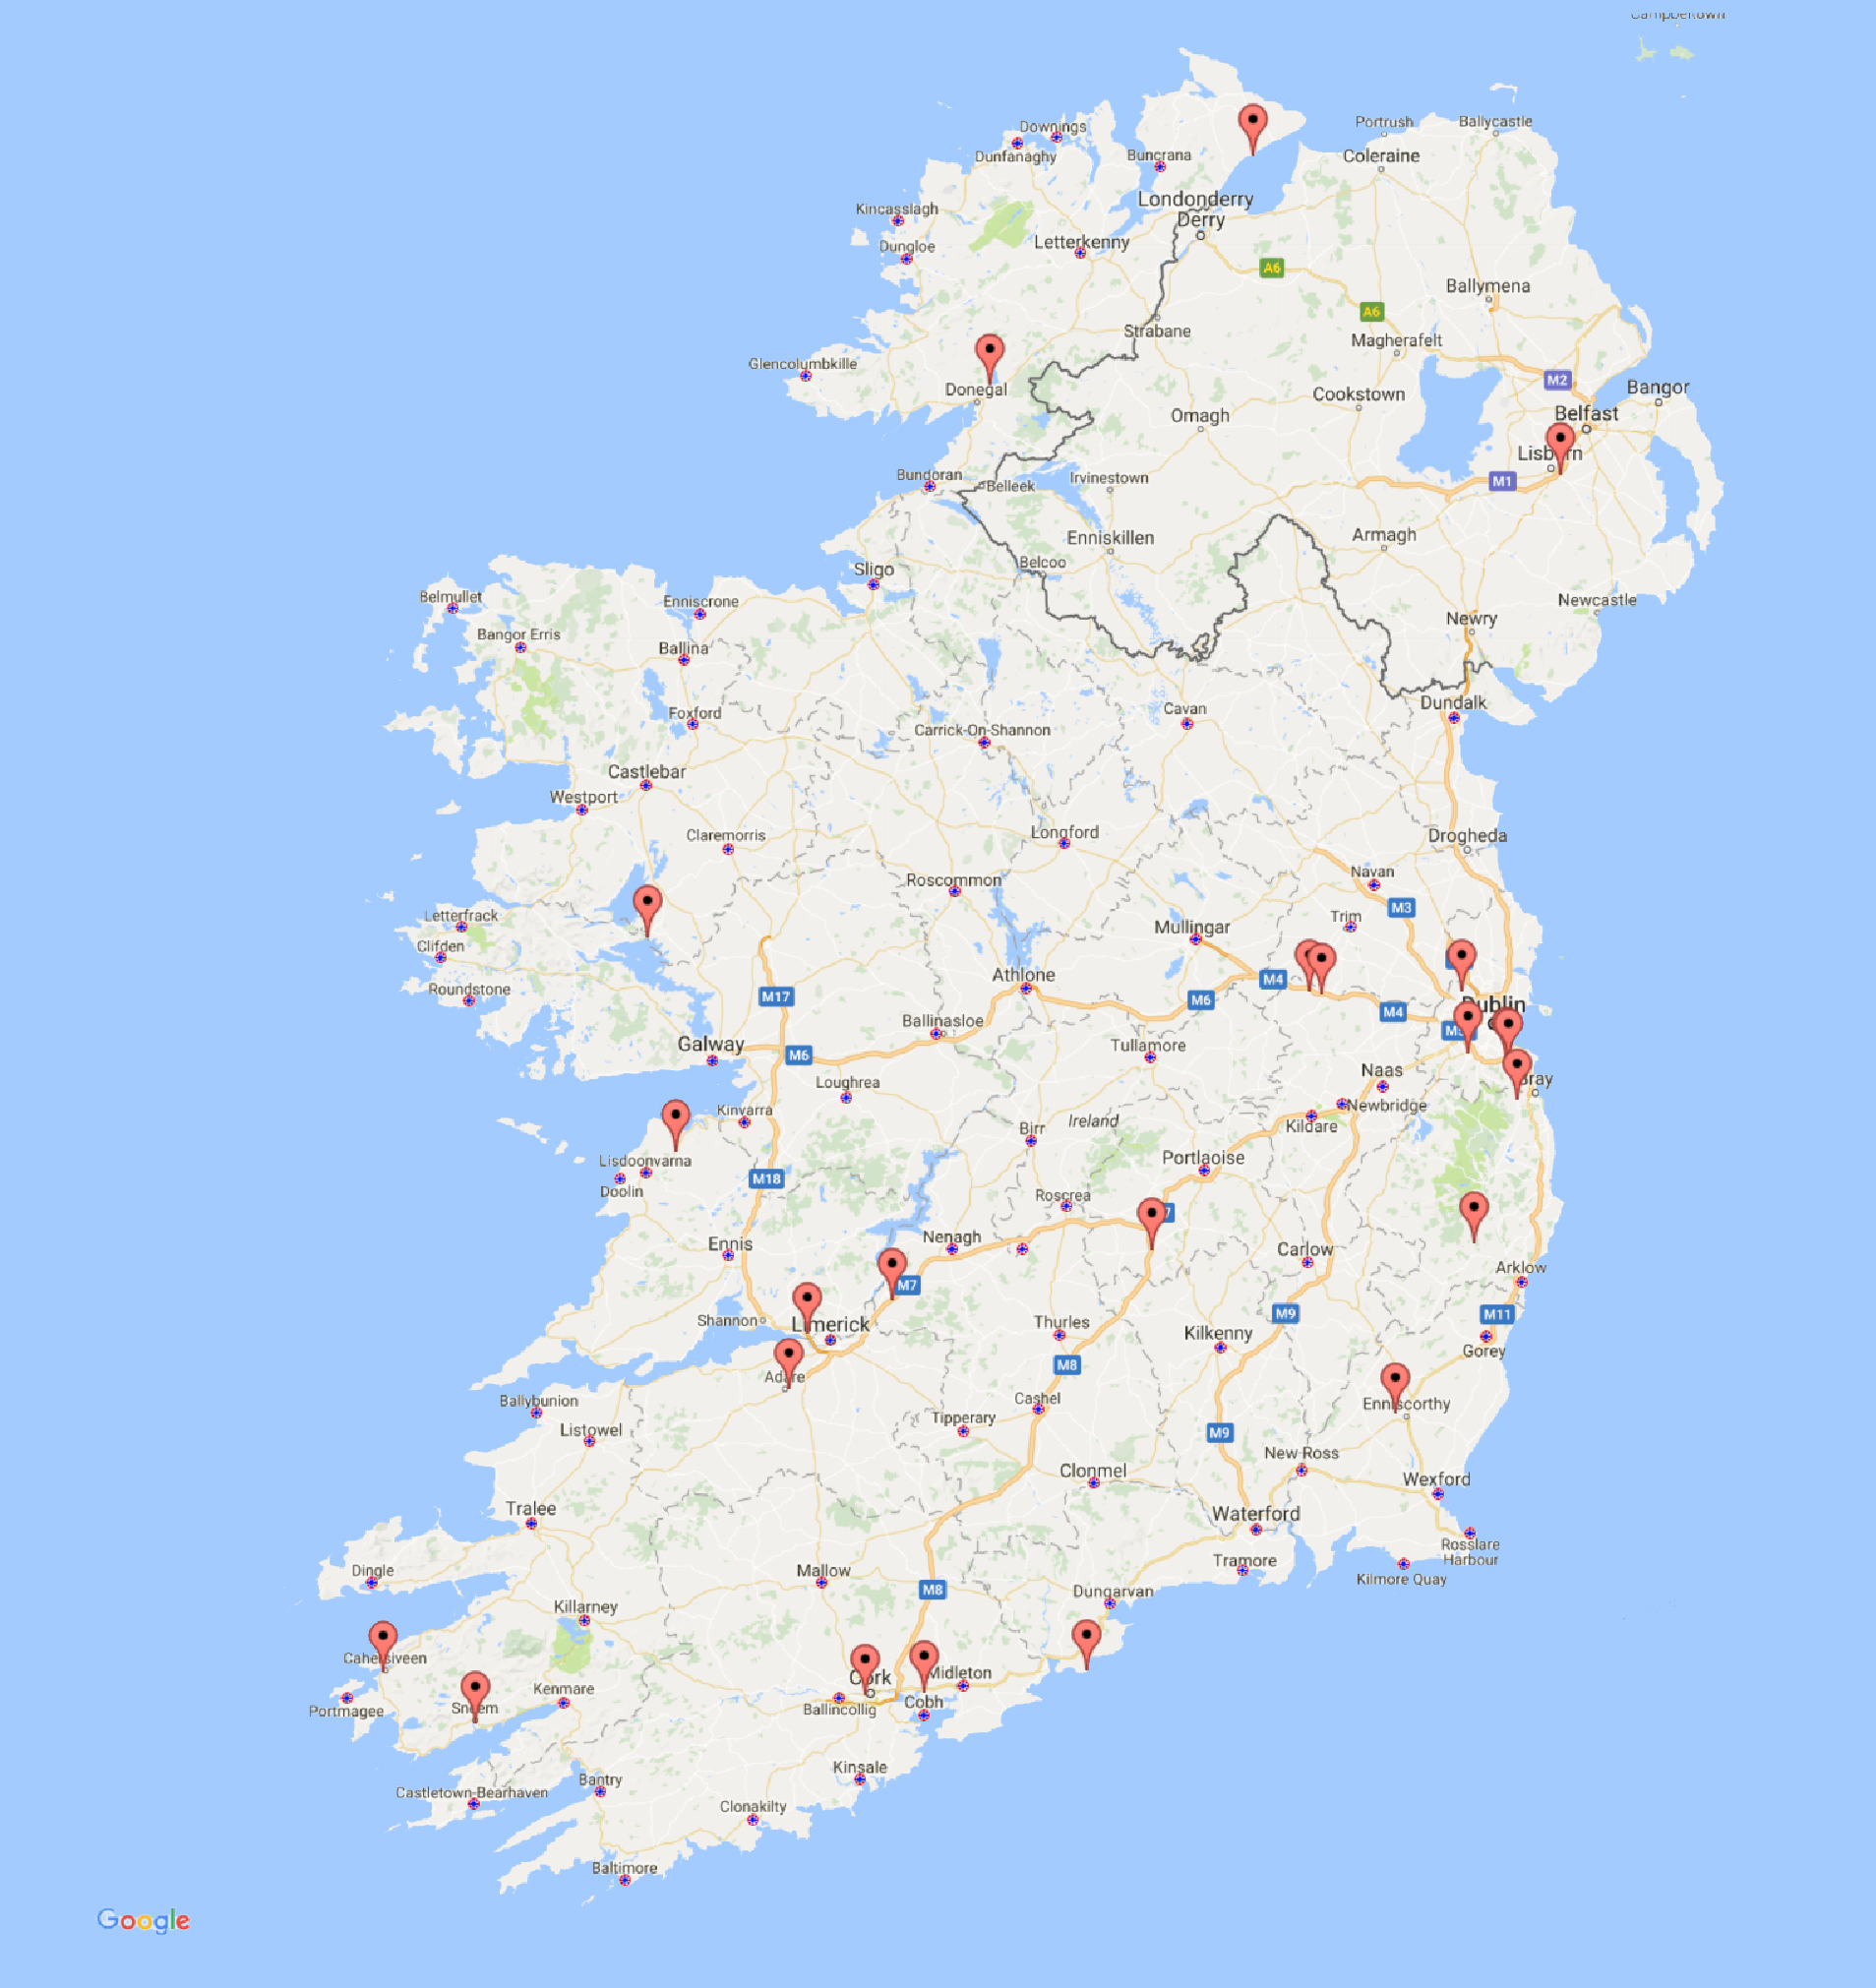
\includegraphics[width=2in]{stage1.pdf}
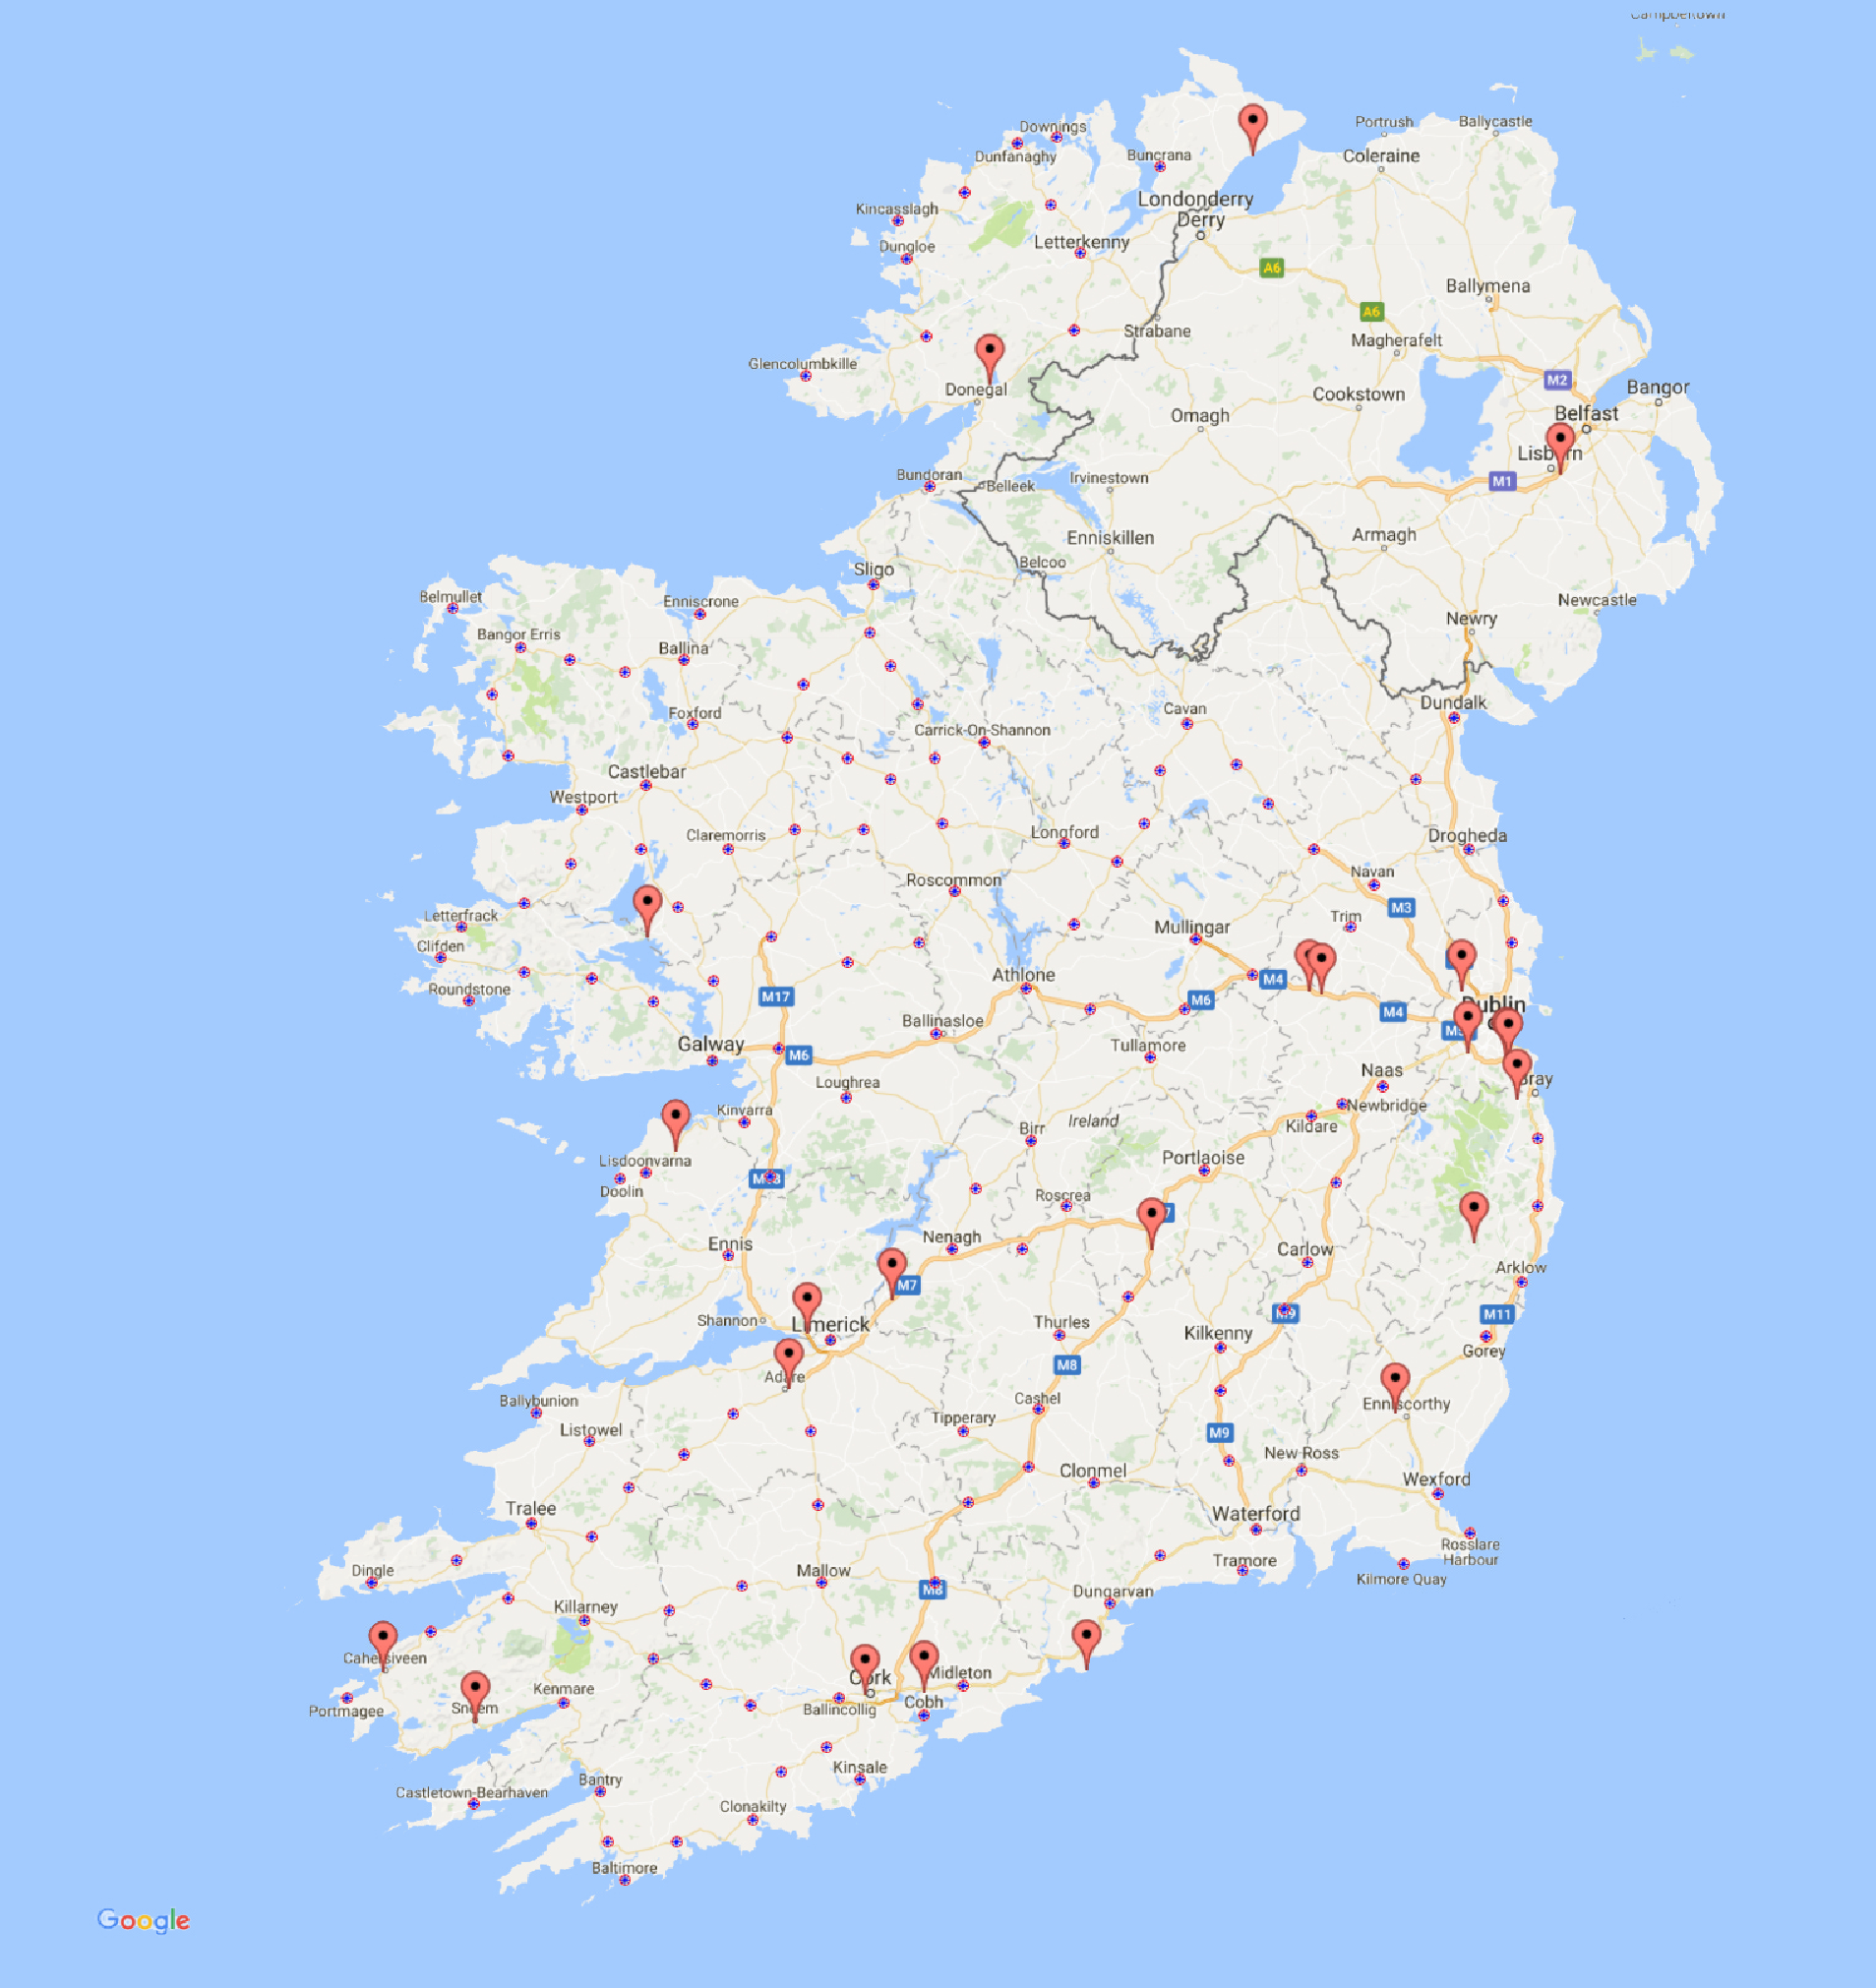
\includegraphics[width=2in]{stage2.pdf}
%\vspace{-0.1in}
\caption{Time evolution of the electric charging station in Ireland.}
\label{fig_stages}
%\vspace{-0.2in}
\end{figure}

We can apply this algorithm to find an optimal solution.
Based on the idea of Greedy Algorithm,
in every iteration,
the algorithm selects nodes in the subgraph induced by $X$ that will not disconnect the subgraph if we delete them from the subgraph.
Then we try to deselect the node with the highest cost $c_j, j \in N_{temp}$.
If $X^{'}$ meets the constrains in Problem~\ref{pro_optimal},
this algorithm shows that $X^{'}$ is a feasible solution.
Then, it continues to the next iteration.
Otherwise, it removes $j$ from $N_{temp}$,
then it deselect the node with the next highest cost.
The iterations terminate when $N_{temp}$ does not contain any node.
Finally, the output $X$ should be the optimal algorithm.

We apply this algorithm to the target nation (Ireland) 
,and try to find the optimal solution in different rates of electric vehicles.
Figure~\ref{fig_stages} shows the result of it.
We will discuss it later in next Section.

\section{The Extension of Our Model}
\label{sec_extension}
In this section, we extend our model to consider other factors (\eg. time evolution) and discuss how those factors influence our model.

\subsection{The Time Evolution of Charging Station Construction}
\label{time}
When considering the time evolution of the charging station construction, a competition model based on Voltera Equation has been applied. Where the competition relation is given by,

\begin{equation}
\label{competition}
  \frac{d}{dt} N_i = r_i x_i ( 1- \frac{\sum \alpha_{ij}x_j}{K_i})
\end{equation}
Where $N_i$ is the number of a certain specie, $\alpha$ is a second order tensor describing the iteration among different "species". When there are 2 "species", which can be reasonable determined through historical data.

For our case, the problem is reduced to a 2 "species" competing problem. Where we set $N_e,N_t$ as the number of electrical vehicles and traditional vehicles respectively.

Therefore the Lotka-Volterra equations are:

\begin{equation}
\label{competition_2}
\left\{
       \begin{array}{lr}
             \frac{d}{dt} N_e & = r_e N_e ( 1- \frac{N_e+\alpha_{12}N_t}{K_1})\\
             \frac{d}{dt} N_t & = r_t N_t ( 1- \frac{N_t+\alpha_{12}N_e}{K_2})
       \end{array}
\right.
\end{equation}



For simplicity, we assume that the total capacity of charging stations is proportional to the number of electrical vehicles $N_e$, i.e.

\begin{equation}
\label{propor}
  \sum Cap(i) \varpropto N_e
\end{equation}

Which indicates that the construction of charing station can be guided by the time evolution of electric vehicles.

For the case in Ireland, we can predict the evolution process based on Equation~\ref{competition_2}, \
and Figure~\ref{fig_evolution} show the result of our prediction.
\begin{figure}[!t]
\centering
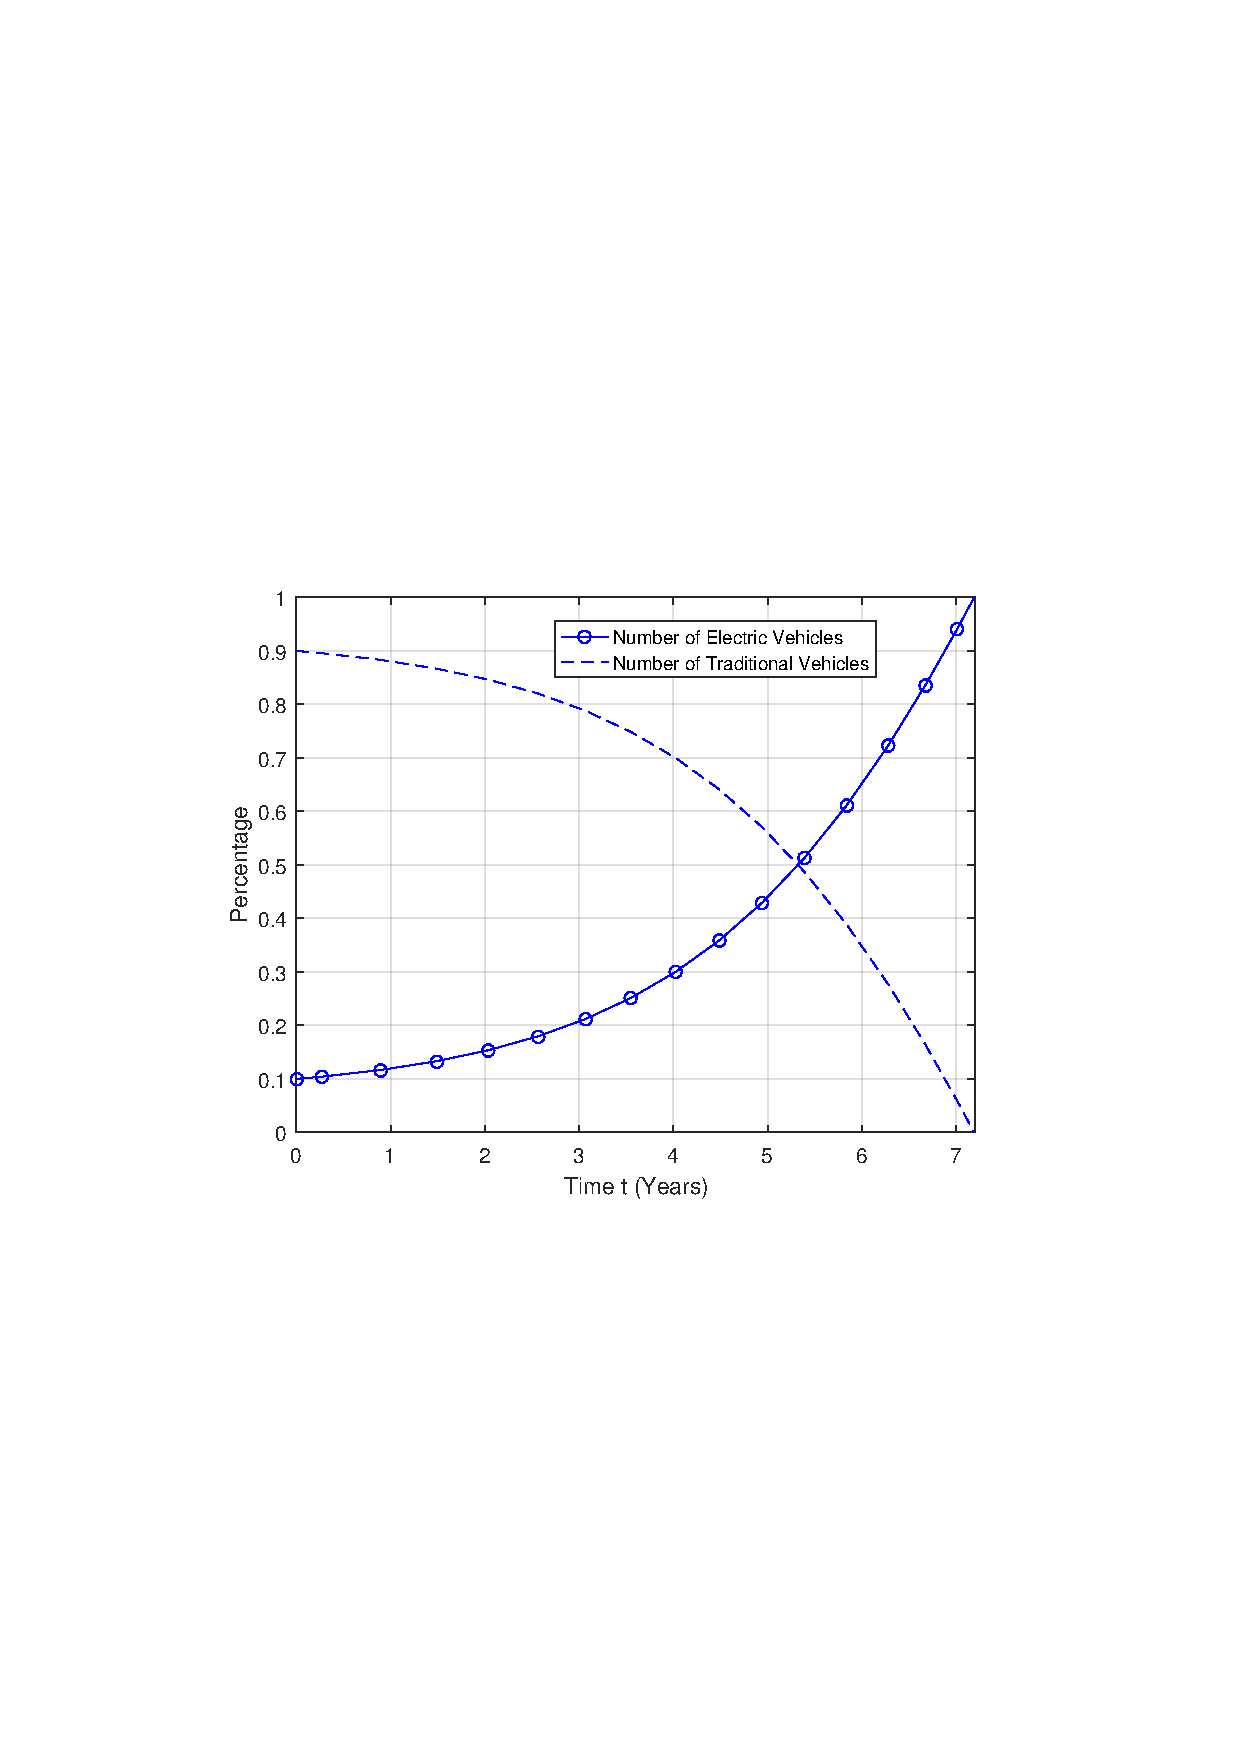
\includegraphics[width=3in]{evolution.pdf}
%\vspace{-0.1in}
\caption{The Evolution Process in Ireland}
\label{fig_evolution}
%\vspace{-0.2in}
\end{figure}
From Figure~\ref{fig_evolution},
we can see that $10\%$

\subsection{City-based Charger, Rural Charger, Population Density Distribution and Wealth Distribution}
\begin{figure}[h]
\centering
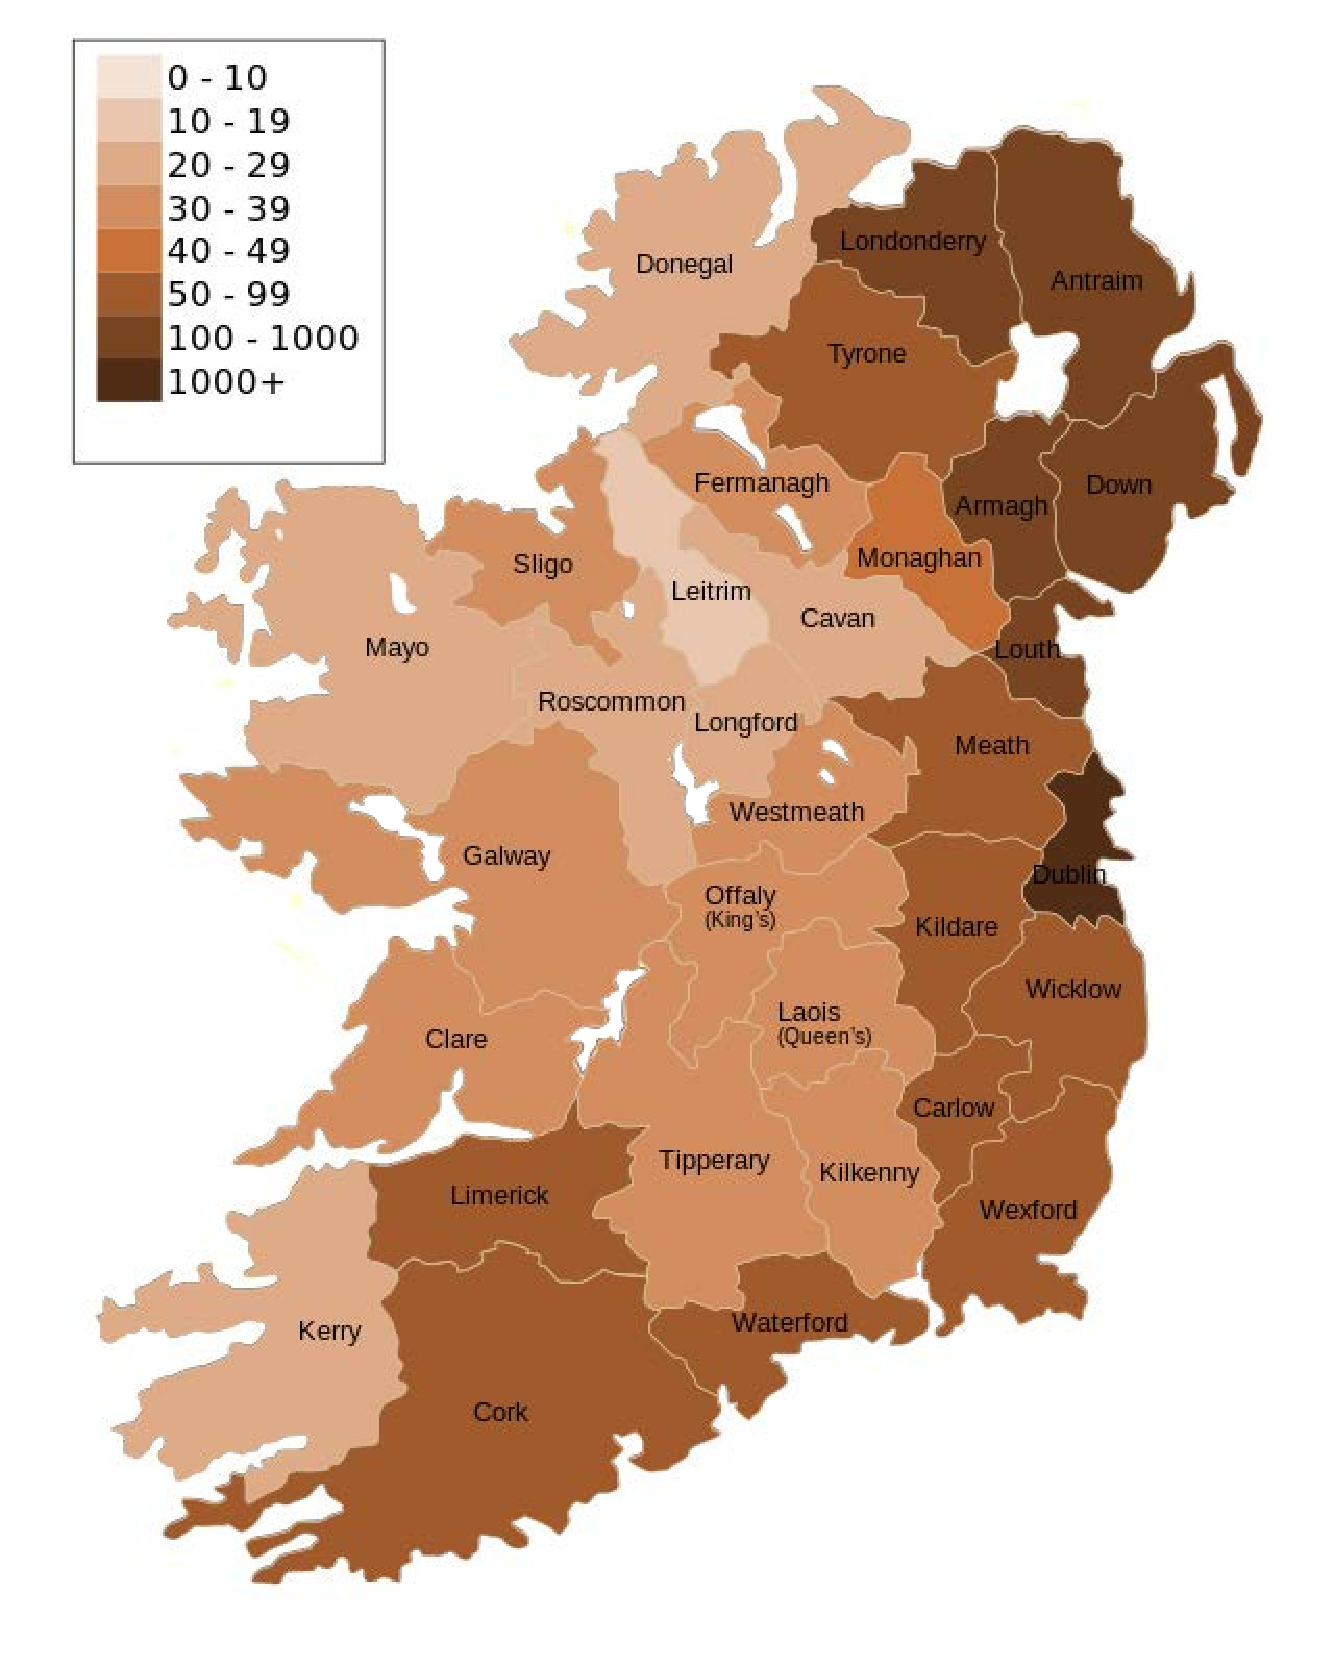
\includegraphics[width=2in]{Ire_Population_Dens.pdf}
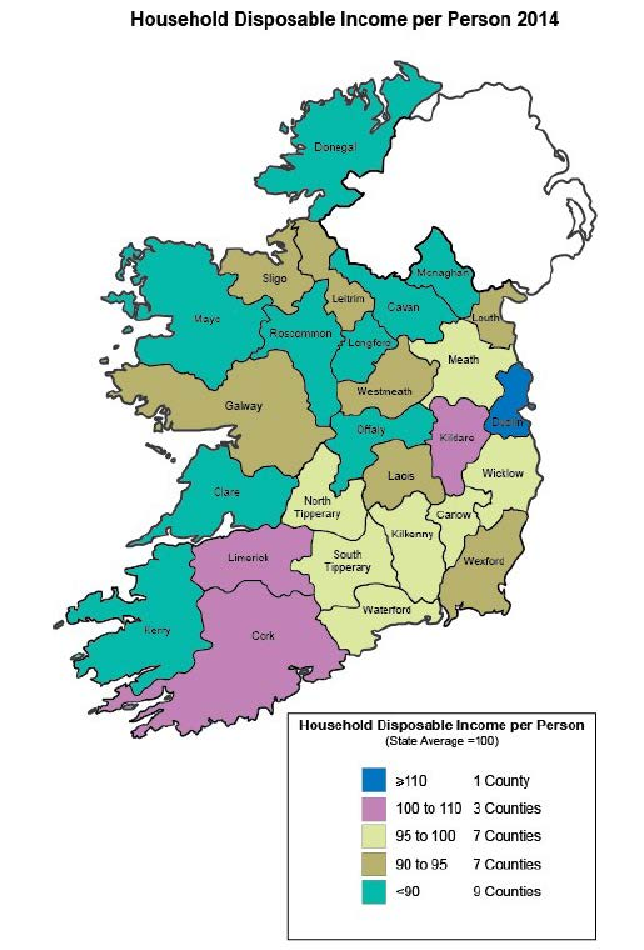
\includegraphics[width=2in]{Ire_wealth.pdf}
%\vspace{-0.1in}
\caption{Interstate difference of Ireland.}
\label{fig_stages_Populatoin}
%\vspace{-0.2in}
\end{figure}



As shown in Figure~\ref{fig_stages} the first stage is the current distribution of charging stations in Ireland.
The algorithm automatically generates the distribution after five years and after a decade, which are stage 2 and 3 respectively.
It shows that the second stage covers most of the cities, villages and towns.
Which is not surprising since not only does the urban area have a higher population density it also has a higher income per capita.
It is also worthy noting that the interstate difference of population density as well as disposable income per household may also impact the time evolution process.

\subsection{Other Transportation Options}
With the development of car-sharing, ride-share services as well as the self-driving cars,
it can be predicted that the information exchanges between charging stations will be greatly increased.
This increasing demand of station-station interaction will consequently stimulates the development of data-sharing network.

The simultaneous data-sharing network system may further enhances the power of electric vehicles from several aspects:
It can both optimize the usage of electric charging station,
shorten the averaged-queueing time and help drivers of the electric vehicles to decide the most reasonable routes when they are traveling from one city to another.

The battery-swap stations may replace the superchargers among the highway since there is no doubt that changing the battery is much more convenient and less time-consuming comparing with stopping at the charging station and waiting for the vehicles to be charged.

Although flying cars and Hyperloops are still prototypes currently, we are quite confident that the rapid development of battery cell will boost the popularization of flying cars and Hyperloops. Noting that the energy consumptions of both flying cars and Hyperloops are relatively high, therefore the electric charing system has to be well planned and established to support these consumptions.

\section{Conclusion}
\label{sec_conclusion}
Considering the problem of the charging station network in the United States,
We find that the charging station network in US cannot support a successful migration towards all'electric personal transportation in the United States,
because there exists the failure case caused by $R_{super} \leq R_{destination}$.
In our model, the total number of charging station support a successful migration towards all'electric personal transportation in the United States  is around 3792,
which is higher than the number of current deployment.

For the problem of determining the optimal number, placement, and distribution in Ireland,
we use the algorithm to find the optimal solution and the result is showed in Figure~\ref{fig_stages}.
We also discuss how other factors (\eg. population distribution, wealth distribution.......) influence our model,
and show the result with various rates of the electric vehicle in Ireland.
We find that those factors mainly shape the first layer in our process architecture.
Thus, the algorithm can also work well in different cases. And the key factors in our model are service capacity $demand(i)$ and the cost of construction $c_i$ in site $i$.  



%%% Feel free to choose any bibliography style you like.
\bibliographystyle{IEEEtrans}
%%% The filename (without the bib extension) of your bibliography file.
\bibliography{icmmcm}

\end{document}
